% Options for packages loaded elsewhere
\PassOptionsToPackage{unicode}{hyperref}
\PassOptionsToPackage{hyphens}{url}
%
\documentclass[
]{article}
\usepackage{amsmath,amssymb}
\usepackage{iftex}
\ifPDFTeX
  \usepackage[T1]{fontenc}
  \usepackage[utf8]{inputenc}
  \usepackage{textcomp} % provide euro and other symbols
\else % if luatex or xetex
  \usepackage{unicode-math} % this also loads fontspec
  \defaultfontfeatures{Scale=MatchLowercase}
  \defaultfontfeatures[\rmfamily]{Ligatures=TeX,Scale=1}
\fi
\usepackage{lmodern}
\ifPDFTeX\else
  % xetex/luatex font selection
\fi
% Use upquote if available, for straight quotes in verbatim environments
\IfFileExists{upquote.sty}{\usepackage{upquote}}{}
\IfFileExists{microtype.sty}{% use microtype if available
  \usepackage[]{microtype}
  \UseMicrotypeSet[protrusion]{basicmath} % disable protrusion for tt fonts
}{}
\makeatletter
\@ifundefined{KOMAClassName}{% if non-KOMA class
  \IfFileExists{parskip.sty}{%
    \usepackage{parskip}
  }{% else
    \setlength{\parindent}{0pt}
    \setlength{\parskip}{6pt plus 2pt minus 1pt}}
}{% if KOMA class
  \KOMAoptions{parskip=half}}
\makeatother
\usepackage{xcolor}
\usepackage[margin=1in]{geometry}
\usepackage{graphicx}
\makeatletter
\def\maxwidth{\ifdim\Gin@nat@width>\linewidth\linewidth\else\Gin@nat@width\fi}
\def\maxheight{\ifdim\Gin@nat@height>\textheight\textheight\else\Gin@nat@height\fi}
\makeatother
% Scale images if necessary, so that they will not overflow the page
% margins by default, and it is still possible to overwrite the defaults
% using explicit options in \includegraphics[width, height, ...]{}
\setkeys{Gin}{width=\maxwidth,height=\maxheight,keepaspectratio}
% Set default figure placement to htbp
\makeatletter
\def\fps@figure{htbp}
\makeatother
\setlength{\emergencystretch}{3em} % prevent overfull lines
\providecommand{\tightlist}{%
  \setlength{\itemsep}{0pt}\setlength{\parskip}{0pt}}
\setcounter{secnumdepth}{-\maxdimen} % remove section numbering
\ifLuaTeX
  \usepackage{selnolig}  % disable illegal ligatures
\fi
\usepackage{bookmark}
\IfFileExists{xurl.sty}{\usepackage{xurl}}{} % add URL line breaks if available
\urlstyle{same}
\hypersetup{
  pdftitle={To Run or Not to Run},
  pdfauthor={Justin C. Eldridge, Chandler Grote, Gabe Macklem},
  hidelinks,
  pdfcreator={LaTeX via pandoc}}

\title{To Run or Not to Run}
\usepackage{etoolbox}
\makeatletter
\providecommand{\subtitle}[1]{% add subtitle to \maketitle
  \apptocmd{\@title}{\par {\large #1 \par}}{}{}
}
\makeatother
\subtitle{Using Pre-Snap Behavior to Predict Play Types in the NFL}
\author{Justin C. Eldridge, Chandler Grote, Gabe Macklem}
\date{2024-12-05}

\begin{document}
\maketitle

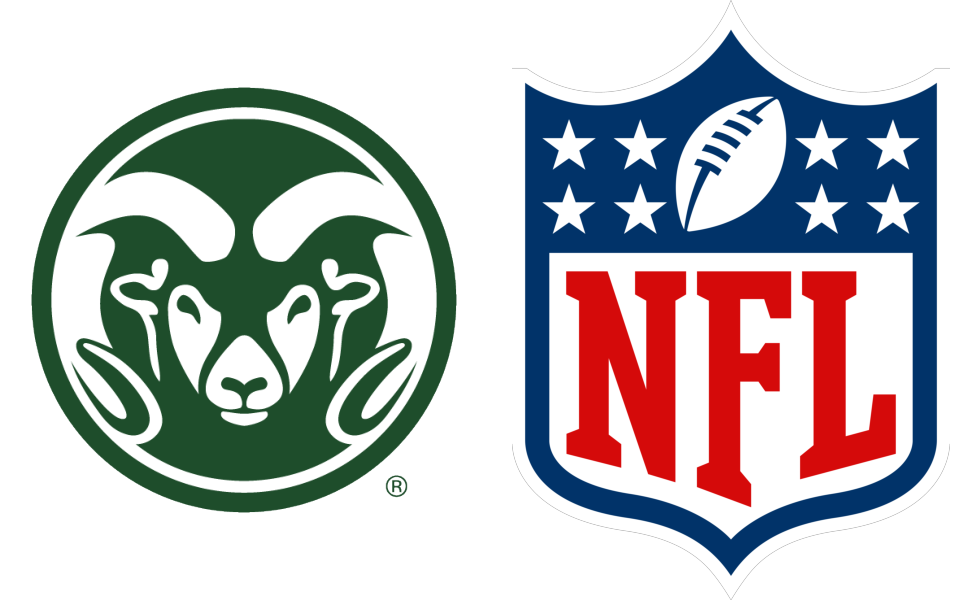
\includegraphics{Paper-RD_files/figure-latex/unnamed-chunk-1-1.pdf}
\newpage

\section{Contents:}\label{contents}

\begin{enumerate}
\def\labelenumi{\arabic{enumi}.}
\tightlist
\item
  Overview/ Introduction
\item
  Description of Data Sets
\item
  Exploratory Data Analysis
\item
  Variables and Data Cleaning
\item
  Model Selection
\item
  Model Evaluation Metrics
\item
  Results- Logistic Regression
\item
  Results- Linear Support Vector Machine
\item
  Results- Random Forrest
\item
  Model Comparison
\item
  Conclusion
\item
  Discussion and Future Research
\item
  Citations
\end{enumerate}

\subsection{1. Overview/ Introduction:}\label{overview-introduction}

For our project we decided to participate in the National Football
League's Big Data Bowl competition for 2025. The purpose of this
competition is to use player and team behavior right before the play
begins to gain insight into the resulting play. We realized that the
most important information a defense can have is whether the offense
intends to execute a run or pass play. Knowing this information would
allow the defensive team to move their players around to optimize their
chances of getting a tackle or otherwise disrupting the play. We
therefore decided to develop statistical models that can predict what
kind of play the offense will execute based on game characteristics,
team characteristics, and player behavior before and during the snap
which we will explore in greater detail later on.

\subsection{2. Data Sets:}\label{data-sets}

The NFL provided several useful data sets for us to draw from for our
analysis.

-\textbf{games.csv}: This set contains all of the game data for the
first 9 weeks of the 2022 season.

-\textbf{plays.csv}: This set contains all of the play by play data.

-\textbf{players.csv}: This set contains all of the individual
performance data for NFL players.

-\textbf{player\_play.csv}: This set contains all of the player level
stats for each game and play.

-\textbf{tracking\_week\_{[}week{]}.csv}: This set contains all of the
tracking data for players and the ball for each game and play in a given
week.

\newpage

\subsection{3. Exploratory Data
Analysis:}\label{exploratory-data-analysis}

Since we were interested to see if things like player motion before or
during the snap could be useful in predicting the play type we decided
to look at a week of tracking data which contains key pre-snap events
like when the offensive line is set (line\_set), when the ball is
snapped (ball\_snap), and whether or not a player was in motion before
the snap (man\_in\_motion) and plot the frequency of these events.

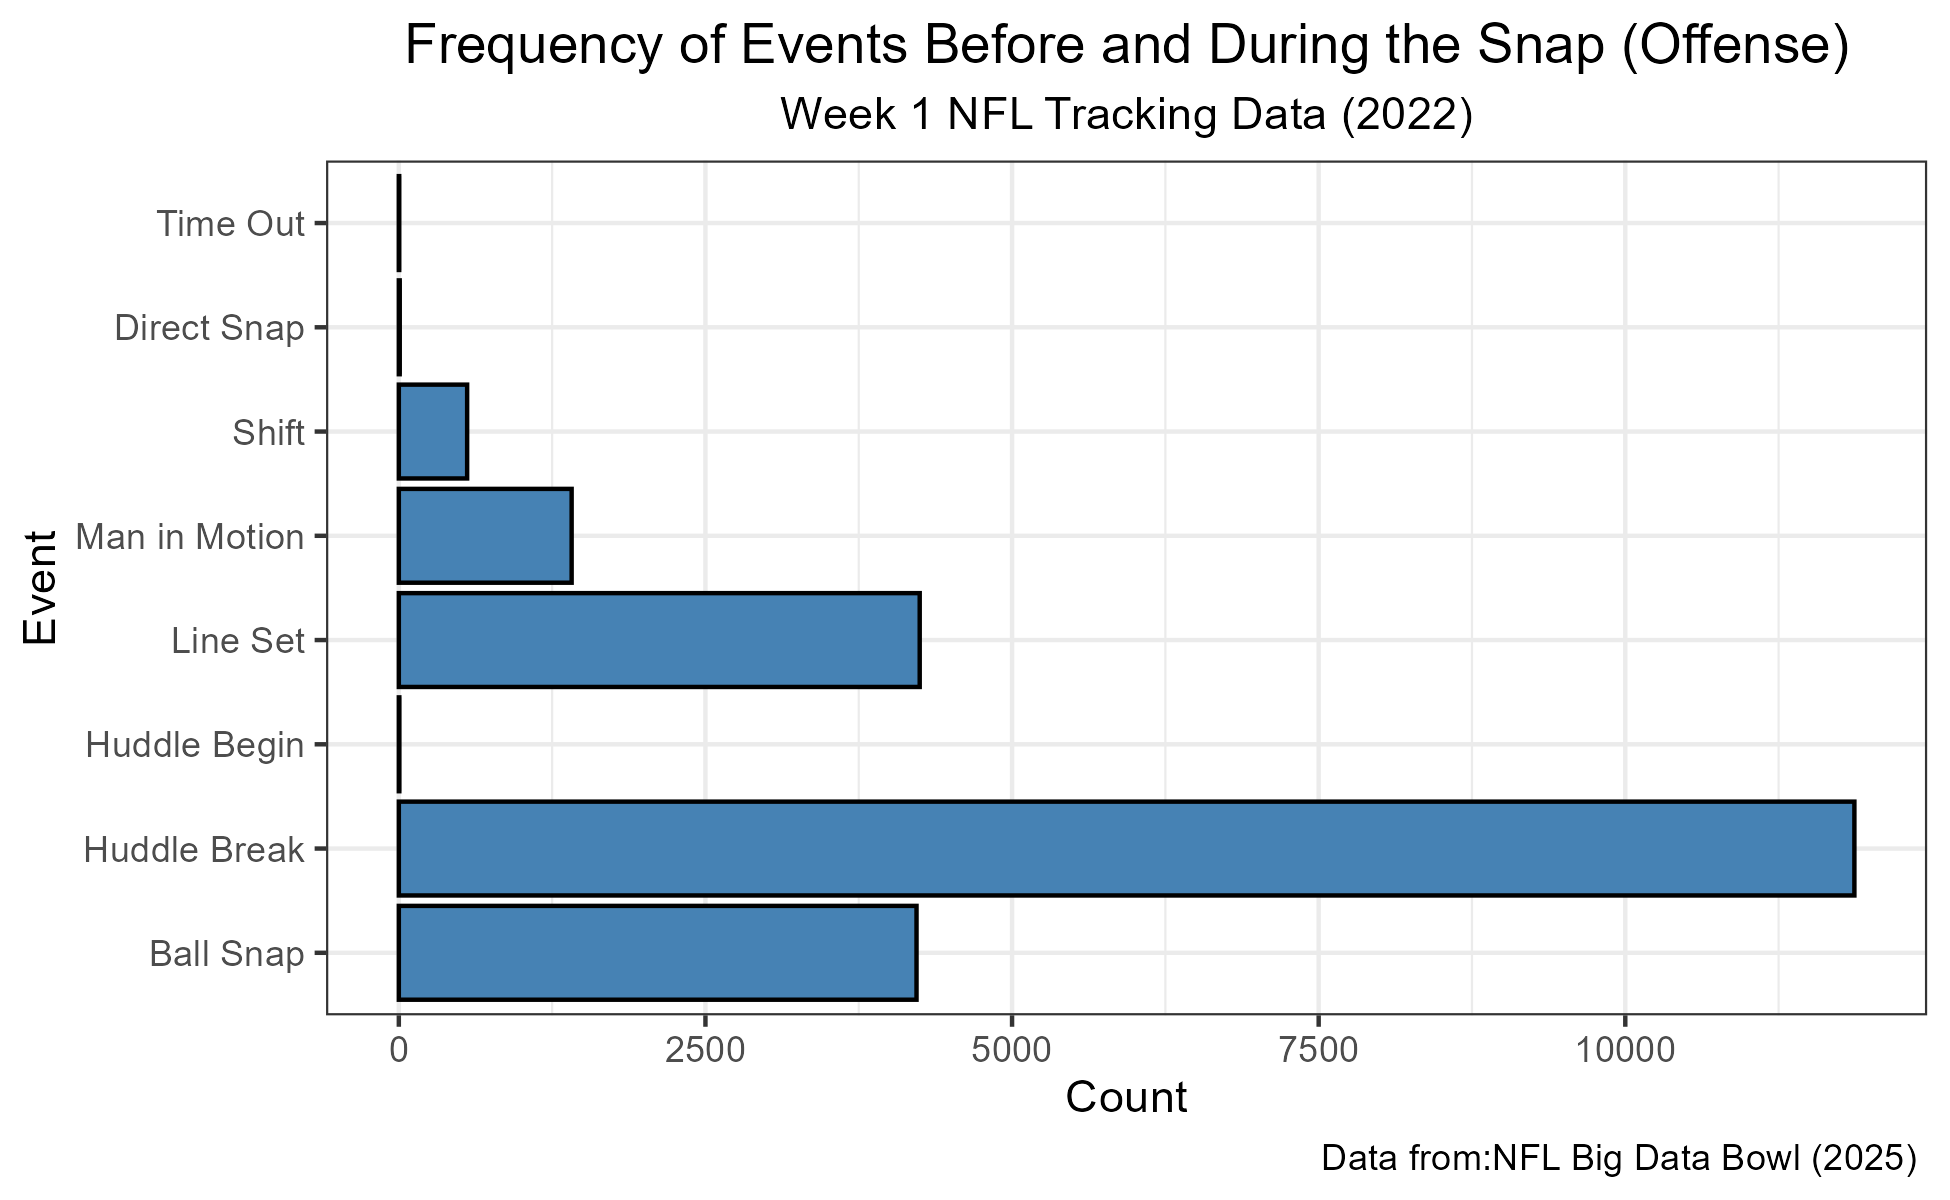
\includegraphics[width=27.08in]{graphs/Images for paper/event_frequency_EDA}
\newpage

We were also interested to know if there would be any imbalance in our
data (i.e.~differing numbers of pass and run plays). To determine this
we created indicator variables that classified any play with a dropback
type of DESIGNED\_RUN, and QB\_SNEAK as a run play and any plays with a
dropback type of TRADITIONAL, SCRAMBLE, or some form of ROLLOUT as pass
plays. We then plotted the frequency of each type to visualize any
imbalance.

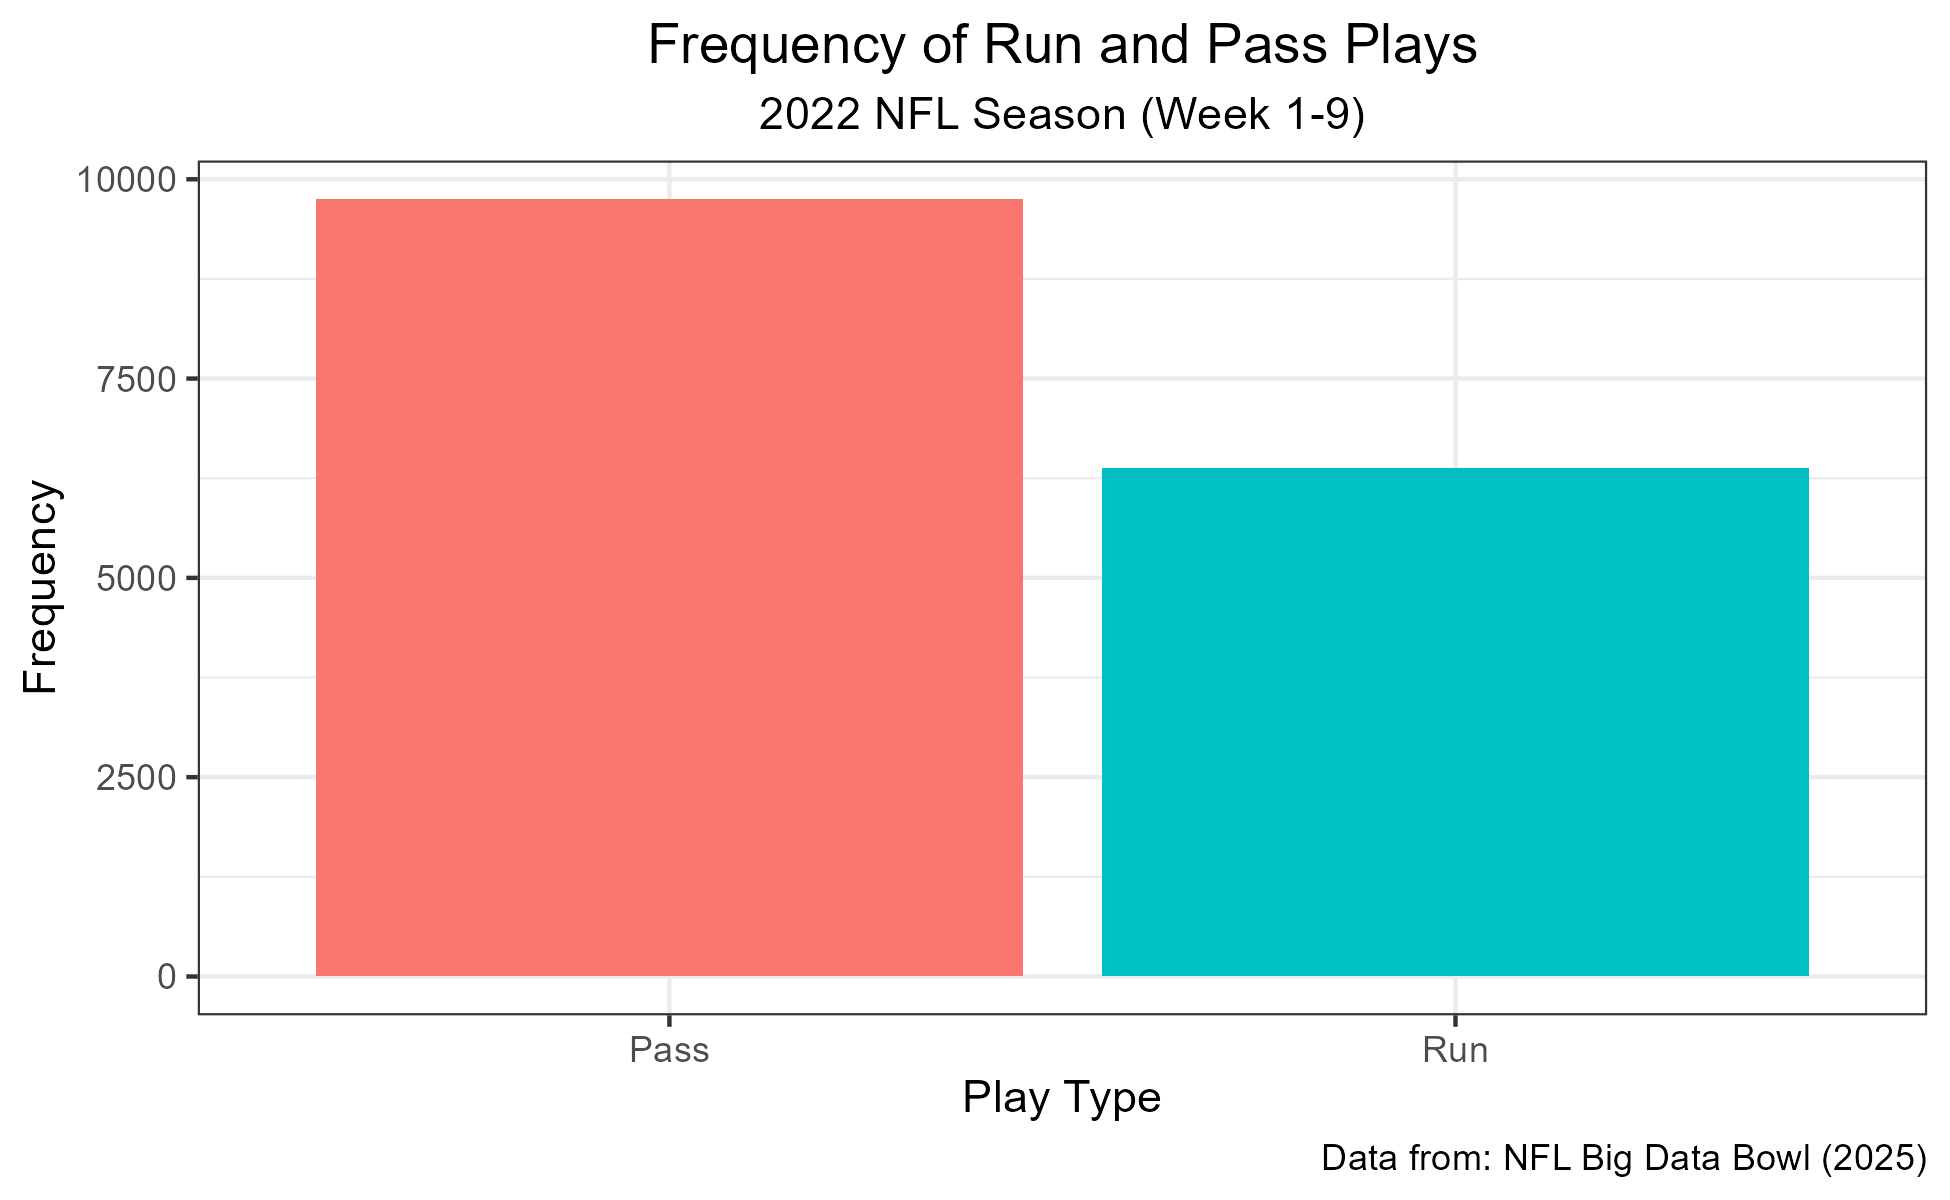
\includegraphics[width=27.08in]{graphs/Images for paper/play_type_frequency_EDA}

Digging deeper, we can observe these trends on a team-by-team basis. We
found that most NFL teams pass more than they run. However, four teams
deviate from this pattern, running more than they pass. Even in these
cases, the difference between run and pass plays is not as drastic as it
is for pass-heavy teams.

\includegraphics[width=27.08in]{graphs/Images for paper/final_AFC_prop}
\includegraphics[width=27.08in]{graphs/Images for paper/final_NFC_prop}

\newpage

\subsection{4. Variables and Data
Cleaning:}\label{variables-and-data-cleaning}

Using our background knowledge and drawing on our EDA we decided to
include the following variables in our models.

\textbf{\emph{Game Characteristics:}}

\begin{itemize}
\tightlist
\item
  \textbf{\texttt{game\_id}}: Unique identifier for the game
\item
  \textbf{\texttt{play\_id}}: Unique identifier for a specific play
\item
  \textbf{\texttt{possession\_team}}: Identifies the offensive team
\item
  \textbf{\texttt{week}}: Identifies which week of the season the game
  was in
\item
  \textbf{\texttt{run\_pass}}: Indicates if the play was a run or a pass
  (response variable)
\item
  \textbf{\texttt{down}}: Identifies which down the offensive team was
  on for a particular play
\item
  \textbf{\texttt{yards\_to\_go}}: The number of yards needed to get a
  first down
\item
  \textbf{\texttt{yards\_to\_endzone}}: The number of yards to the
  opponent's endzone
\item
  \textbf{\texttt{redzone}}: Indicates whether the offense is within 20
  yards of the opponent's endzone
\item
  \textbf{\texttt{sec\_in\_half}}: The number of seconds remaining on
  the play clock in the current half
\item
  \textbf{\texttt{epa\_lag}}: Serial correlation of expected points
  added
\end{itemize}

Many of these were generated by the NFL but some of them were made by us
using their provided data set. The run\_pass indicator we used as our
response was a classification made by us within the data as they did not
provide a strict column for run or pass. The epa\_lag variable was also
generated using the provided expectedPointsAdded column. The lag is done
on a per drive basis and every new drive of an offense starts at
epa\_lag = 0. We felt the indication of previous play success (positive
epa) would be a significant contributor to the prediction models.

\textbf{\emph{Team Characteristics:}}

\begin{itemize}
\tightlist
\item
  \textbf{\texttt{offense\_formation}}: Categorical variable indicating
  what formation the offense uses
\item
  \textbf{\texttt{receiver\_alignment}}: Enumerated as 0x0, 1x0, 1x1,
  2x0, 2x1, 2x2, 3x0, 3x1, 3x2 (text)
\item
  \textbf{\texttt{curr\_win\_percentage}}: Win percentage for the
  current offensive team
\item
  \textbf{\texttt{form\_change}}: Uses shifts to determine if the
  offense changed formation before the ball was snapped
\end{itemize}

These variables all came from the provided data set. These were some
characteristics we felt would positively contribute to the prediction
models as they relate to overall team by team trends. We knew the models
would be broken up by team as each team has their own offensive
philosophies and as such these would show those tendencies.

\textbf{\emph{Player Characteristics:}}

\begin{itemize}
\tightlist
\item
  \textbf{\texttt{wr\_motion}}: Indicates if a wide receiver moved after
  the line was set
\item
  \textbf{\texttt{te\_motion}}: Indicates if a tight end moved after the
  line was set
\item
  \textbf{\texttt{rb\_motion}}: Indicates if a running back moved after
  the line was set
\item
  \textbf{\texttt{wr\_atsnap}}: Indicates if a wide receiver was in
  motion at the time of the snap
\item
  \textbf{\texttt{te\_atsnap}}: Indicates if a tight end was in motion
  at the time of the snap
\item
  \textbf{\texttt{rb\_atsnap}}: Indicates if a running back was in
  motion at the time of the snap
\end{itemize}

These are the variables incorporating the player tracking data.
Initially we were trying to condense the large week by week tracking
csv's in order to get these important predictors. However, we found that
the NFL actually provided a condensed version of those tracking files to
us, and we were able to generate each position a boolean of presnap
motion and at snap motion. We wanted to keep the feature space on these
more generic as a specific wide receiver motion or ``left to right''
indicators would introduce more noise in an already quite large
predictor space.

\subsection{5. Model Selection:}\label{model-selection}

We were interested in predicting the type of play the offense will
execute. We had a large number of predictors and the predictor space was
further increased by our addition of several indicator variables for
player motion. We therefore selected models that are good for binary
classification and those that can handle larger predictor spaces without
taking an excessive amount of time to run. We additionally wanted to try
a non-parametric approach for comparison. We decided to fit models by
teams as there is significant variation in play style and strategy
across the league. For example, we can see from the run pass proportion
graphs that some teams are much more likely to pass in all situations.
This makes sense as teams who have very good quarterbacks are most
likely to utilize pass plays. These considerations lead us to choose the
following models.

\textbf{Logistic Regression (LASSO):}

First we wanted to create a basic logistic regression model as
``control'' that we could compare our other more sophisticated models
against. To accomplish this we used LASSO with 10-fold cross validation
on the entire data set to perform variable selection. Once the optimal
lambda value had been determined and the optimal LASSO model fit we look
at the output to determine which of our variables to include in the
logistic regression model. We then fit the logistic regression model on
the entire data set in an attempt to identify any and all errors that
would occurr later on when we tried to fit models for each team
individually. Once this was complete we then fit a logistic regression
model for each NFL team

\textbf{Linear Support Vector Machine (SVM):}

For the SVM Model we knew that the binary classification power would
work well for our research question. There was a fairly high predictor
space that we just left as and see if it could tackle them all before
reduction would be required. This did take a while in practice and the
k-fold cross validation had to be reduced from 10 folds to just 5 folds.
Even with this reduction in k-folds the model still took quite a while
to complete the training for all 32 teams. However as discussed later
the prediction power of this method was retained and produced quite
favorable results.

\textbf{Random Forest:}

A tree based model, such as a Random Forest, appeared to be a good
method for predicting NFL play outcomes given its nonparametric nature.
The game of football is very complex with many intricate trends that may
be difficult to recognize. Taking into account the many game settings
presented in a NFL game, along with the trends and intricacies of a
complex NFL offense, this model may be able to distinguish between a
potential run or pass.

For testing this method, a model was fit on each NFL team using 7-fold
cross-validation to find the optimal parameters. Given our data set
included the first nine weeks of the NFL season, the primarily assessed
model was trained on the teams first 5-6 games(5 if a team had a bye
week in the early parts of the season) and tested on the final 3 games
of this period.

When training the models, the proportion at which a team runs and passes
was considered. To account for a potential minority class, we calculated
the ratio between the number of cases in the majority class with the
number of cases in the minority class. This value was the weight value
assigned to the minority class. By weighting the minority class, we were
able to assign greater importance to this class when training. Without
this, we may notice greater imbalances in the model's ability to predict
the minority class. The problem we are attempting to answer relies on
this, as predicting a pass or run is equally as important.

\textbf{KNN:}

KNN was a non-parametric approach to the research question we tried. KNN
can prove quite powerful when there is little overlap in the response
compared to the feature space, which was our hope. However that did not
prove to be the case and we ended abandoning this model all together.
Part of the problem for KNN is the number of observations compared to
the dimensionality of the problem. Predicting run or pass is a
complicated endeavor and NFL offenses only get around 60 plays a game.
Even when attempting to run on all 8-9 games for a team, that is only
540 games, or so, per team to train on. The model would run for some but
failed to execute the prediction step for approximately half of the
teams. We tried to make adjustments to the model to get predictions for
every team but it was apparent KNN was not going to be a tool that we
could use to describe the outcome effectively and so we decided to move
on from this approach all together.

\subsection{6. Model Evaluation:}\label{model-evaluation}

To evaluate our models performance we decided to employ Matthews
Correlation Coefficient (MCC). MCC which can be understood as the
correlation coefficient between predicted and actual classifications can
be expressed mathematically as follows:

\[
\text{MCC} = \frac{TP \times TN - FP \times FN}{\sqrt{(TP + FP)(TP + FN)(TN + FP)(TN + FN)}}
\] Here an MCC score of 1 indicates perfect agreement between predicted
classes and actual classes, a score of -1 indicates complete
disagreement between predicted and actual classes, and a score of 0
indicates that the predictions are no better than randomly guessing the
class.

We can see that the numerator rewards true positives and true negatives
while penalizing false positives and false negatives. The deonominator
ensures that MCC scores are normalized between -1 to 1.

We chose to utilize MCC for several reasons. First, MCC is good at
handling imbalanced data, which would be useful considering that pass
plays are meaningfully more frequent than run plays. Second, it is
comprehensive, considering all elements of the confusion matrices.
Finally, we chose MCC because unlike precision and accuracy, MCC is
unbiased.

\subsection{7. Results- Logistic Regression
(LASSO):}\label{results--logistic-regression-lasso}

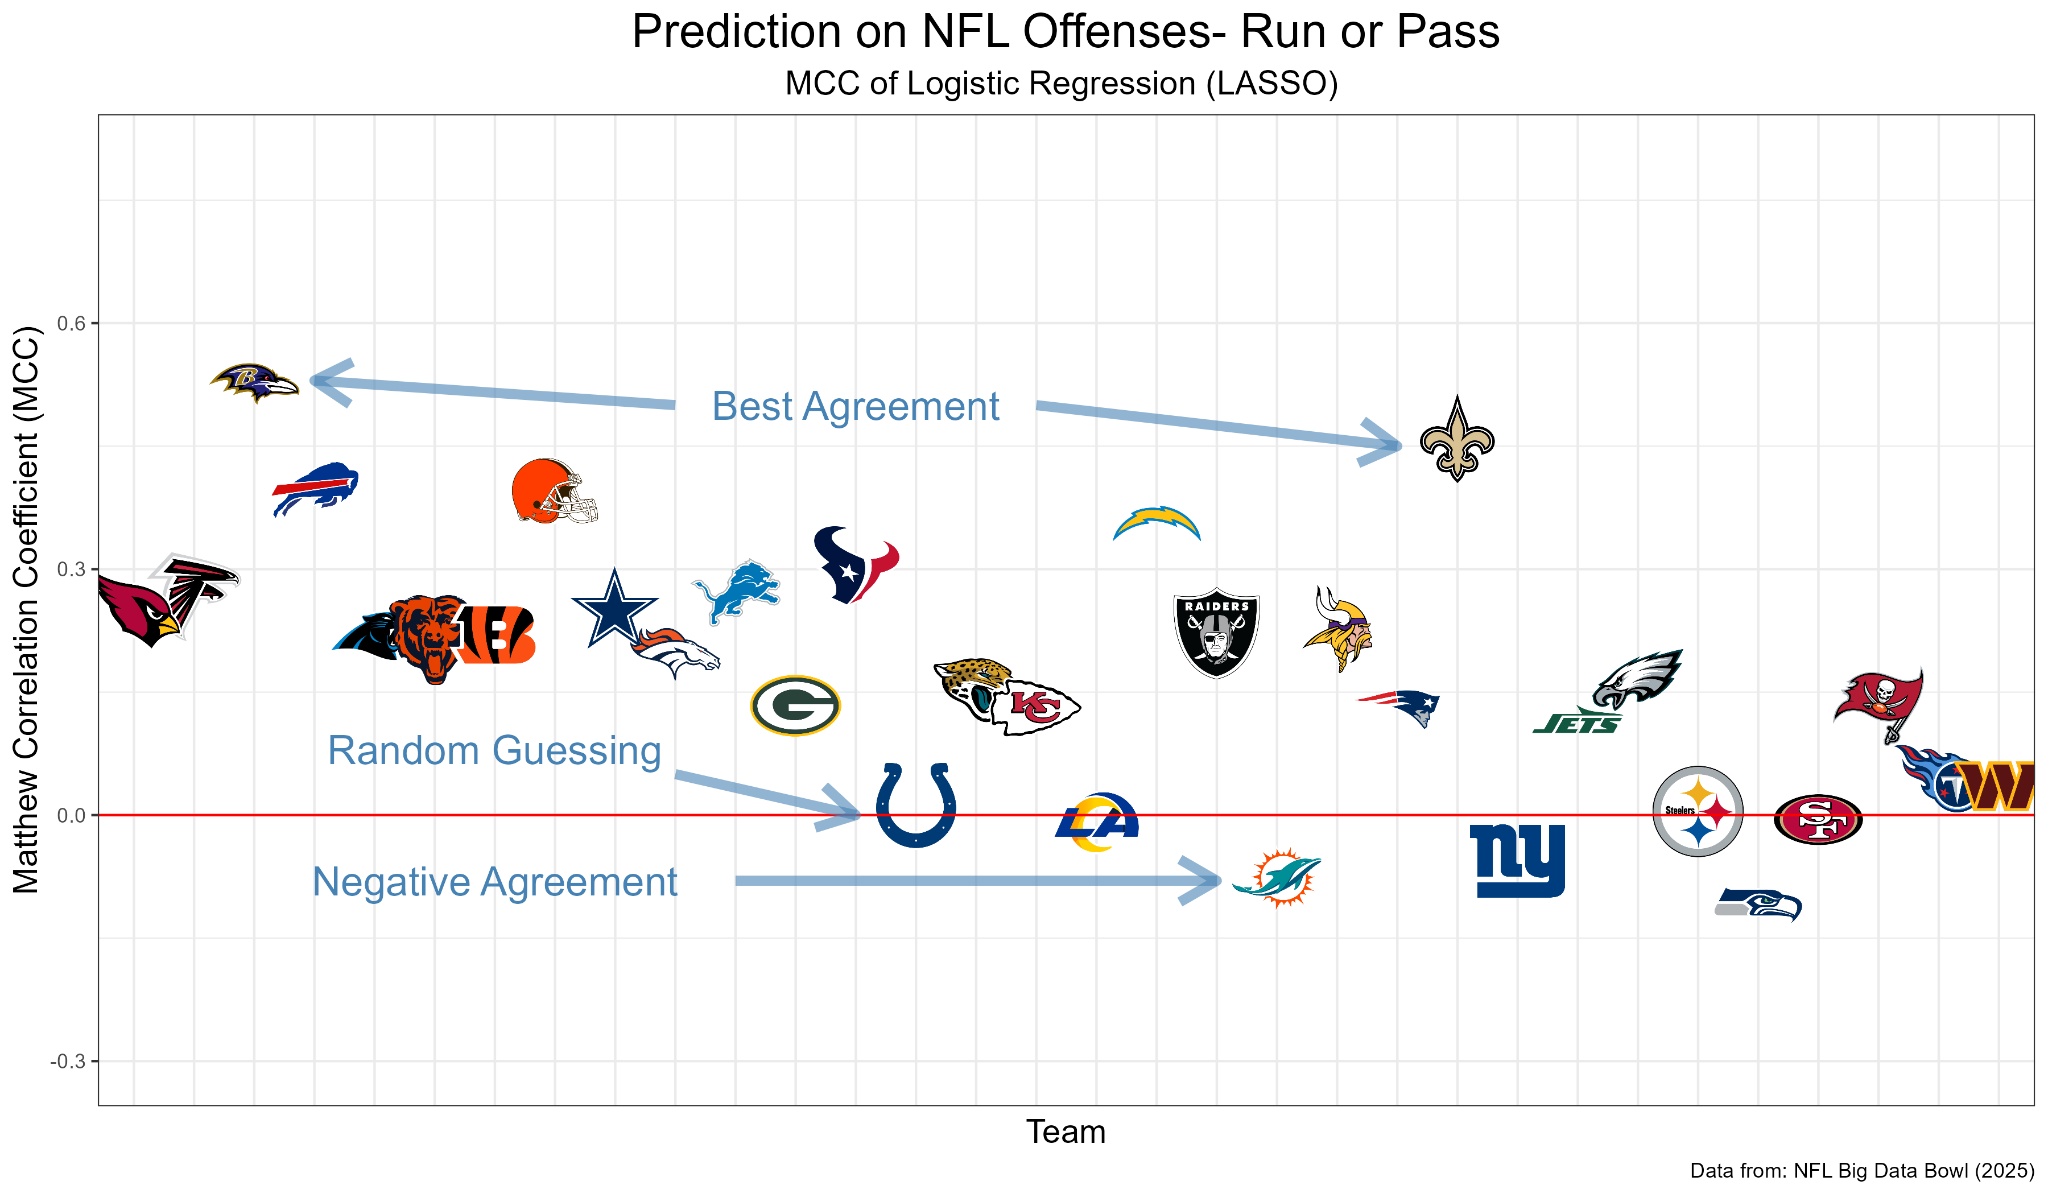
\includegraphics[width=1\textwidth,height=\textheight]{graphs/Images for paper/MCC_Logistic_Original.png}

In the above figure we can see the value of Matthews Correlation
Coefficient for each teams logistic regression model. It is clear that
most of the models showed modest levels of positive agreement between
predictions and reality with the best agreement of \$ 0.53\$ occurring
in the Baltimore Ravens model (top left), and the second best of
\(0.46\) for the New Orleans Saints.

There were also several models with MCC scores of \(\approx 0\). These
teams include the Indianapolis Colts, Los Angeles Rams, Pittsburgh
Steelers, and the San Francisco 49'ers. The MCC score for these models
indicate that their predictions for run or pass were no better than
random guessing.

Finally we can see that three of the models had negative MCC scores,
namely the Miami Dolphins, The New York Giants, and the Seattle
Seahawks. These MCC scores indicate that the models performed even worse
than random guessing.

I have been unable to determine how this happened but I may have made an
error in the logistic model. When I tried to put all of my code for the
logistic model into one file the resulting plot is different from the
one shown above. I cannot say what happened at this stage but I will
include the new version of the plot for comparison.

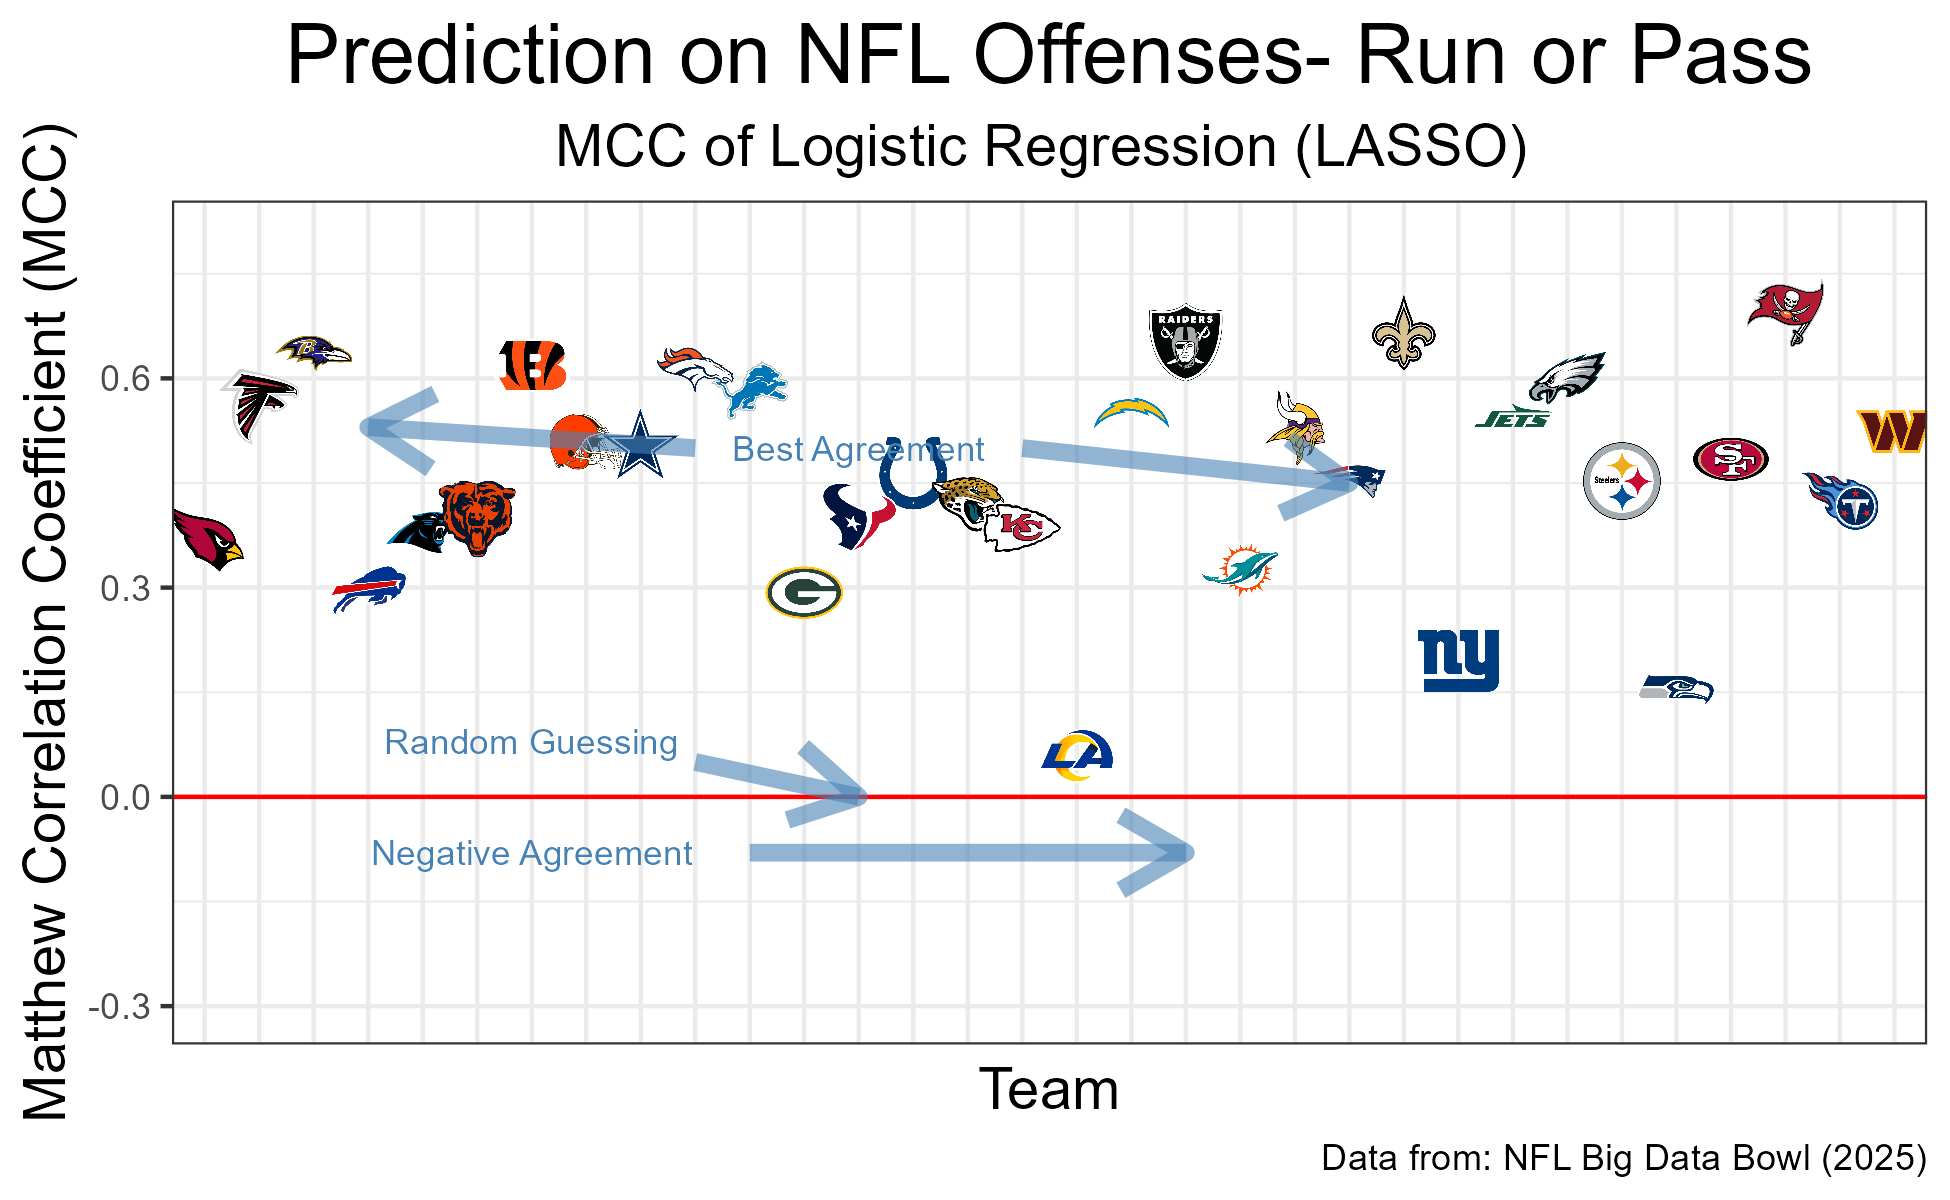
\includegraphics[width=27.08in]{graphs/Images for paper/MCC_log}

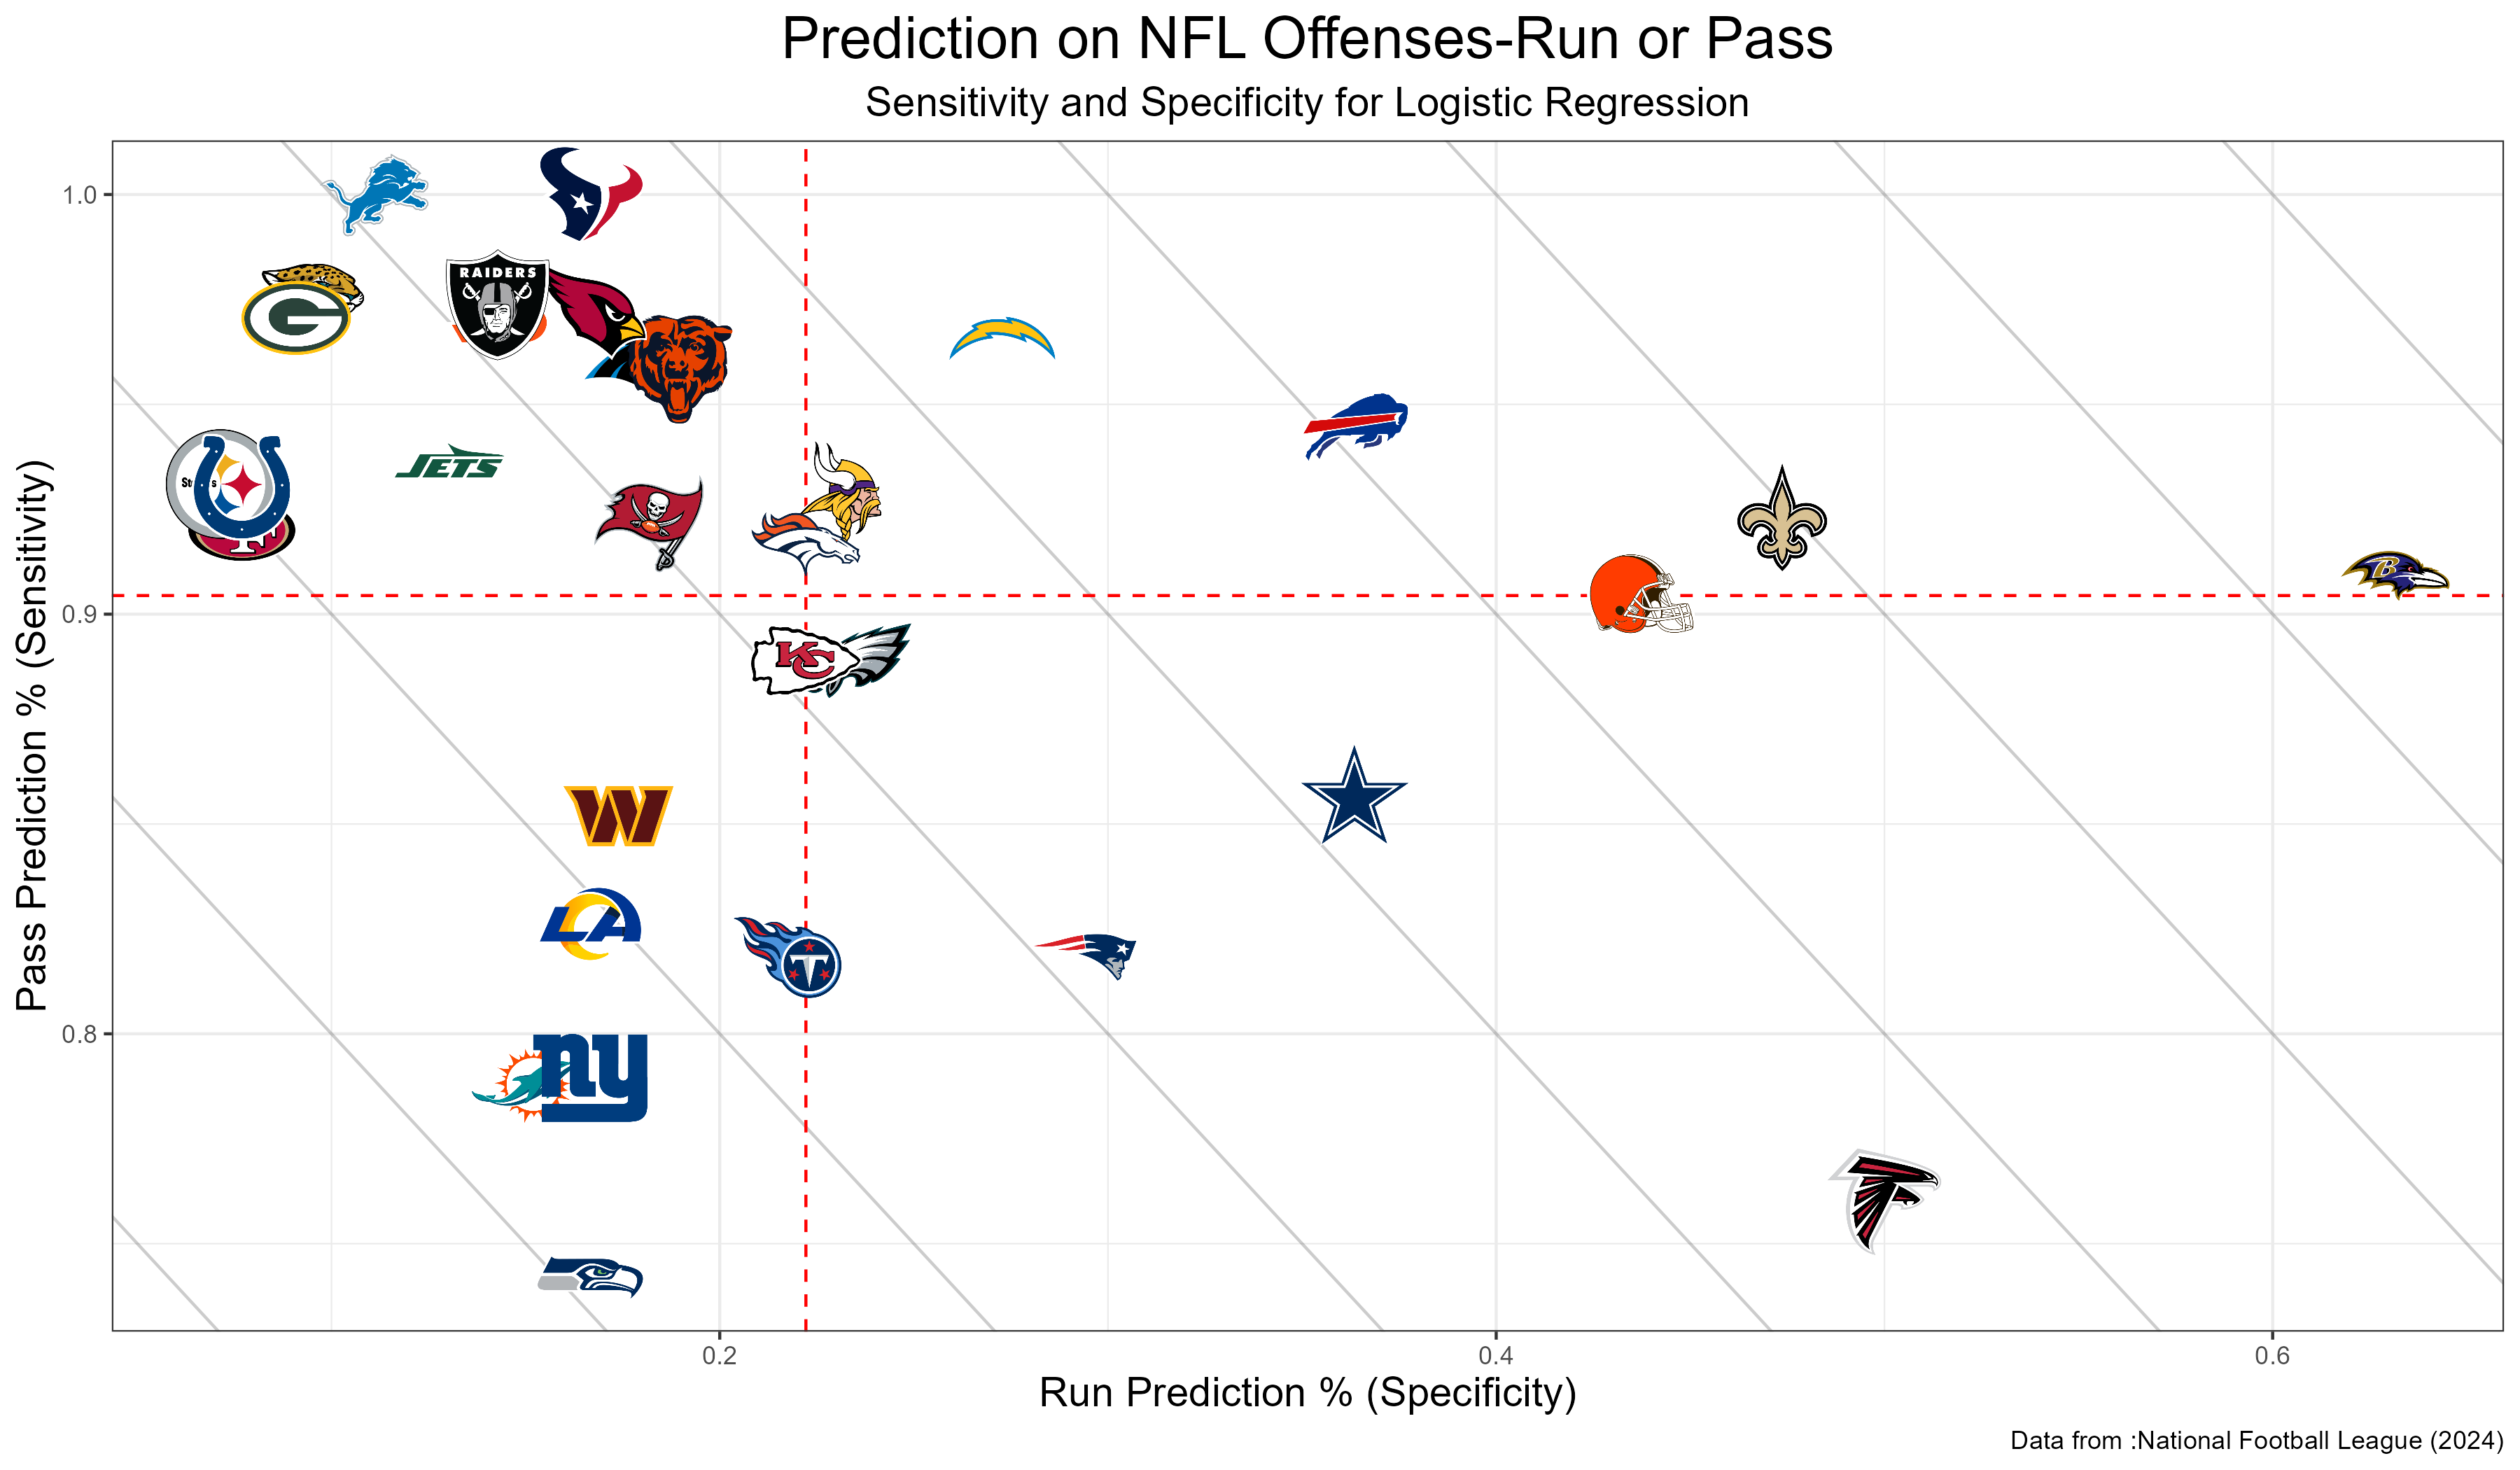
\includegraphics[width=1\textwidth,height=\textheight]{graphs/Sens_vs_spec_Logistic_Original.png}

The above plot shows sensitivity (True Positive Rate) vs.~specificity
(True Negative rate) for each teams logistic regression model. The
dotted red lines represent the mean sensitivity (\(\approx 0.905\)) and
specificity (\(\approx 0.23\)) respectively. These means that the models
were generally biased towards predicting passes, which is consistent
with our earlier findings that pass plays are more common than run
plays. The largest cluster of teams are located in the upper left
quadrant where teams had above-average predictability for passing and
below-average predictability for running. In the bottom left quadrant we
there appears to be a lower bound on predictability for running. There
appears to be much wider variation among teams with above average
predictability for runs shown by the lesser amount of clustering on the
right side of the graph.

As mentioned above when trying to put all of the code for the logistic
model in a single file numeric discrepancies arose that greatly alter
the resulting plots. I have not been able to determine the cause but I
will again include the updated graph for comparison.

\includegraphics[width=27.08in]{graphs/Images for paper/Sens_vs_Spec_log}

\newpage

\subsection{8. Results- Linear SVM:}\label{results--linear-svm}

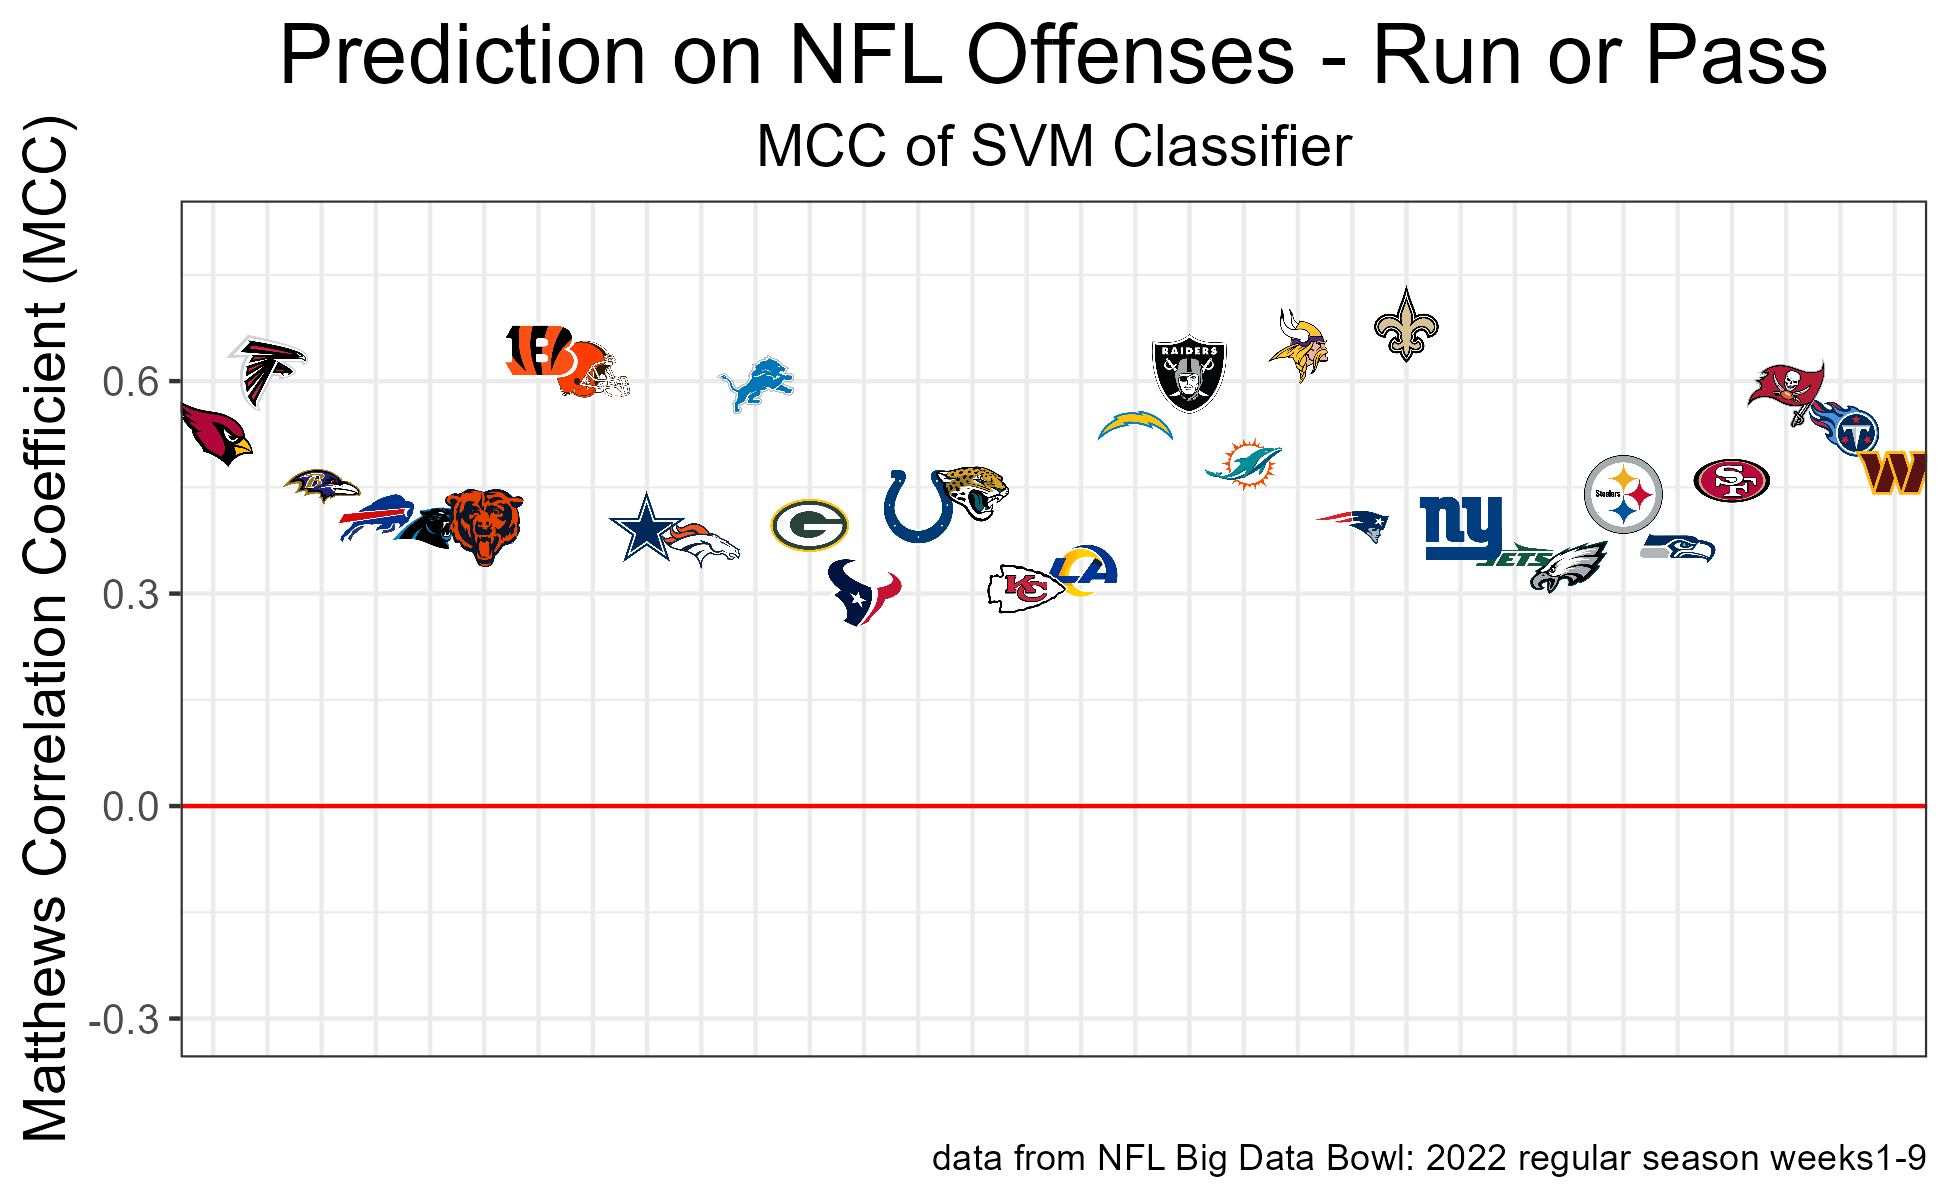
\includegraphics[width=27.08in]{graphs/Images for paper/MCC for SVM}

SVM performed well in terms of classification using the MCC. In the MCC
plot for each team we see a band around 0.3 to 0.7 that each team lives
in. Some are higher than others but all of them are above 0 indicating
the SVM model performed quite well at predicting run or pass.

\newpage

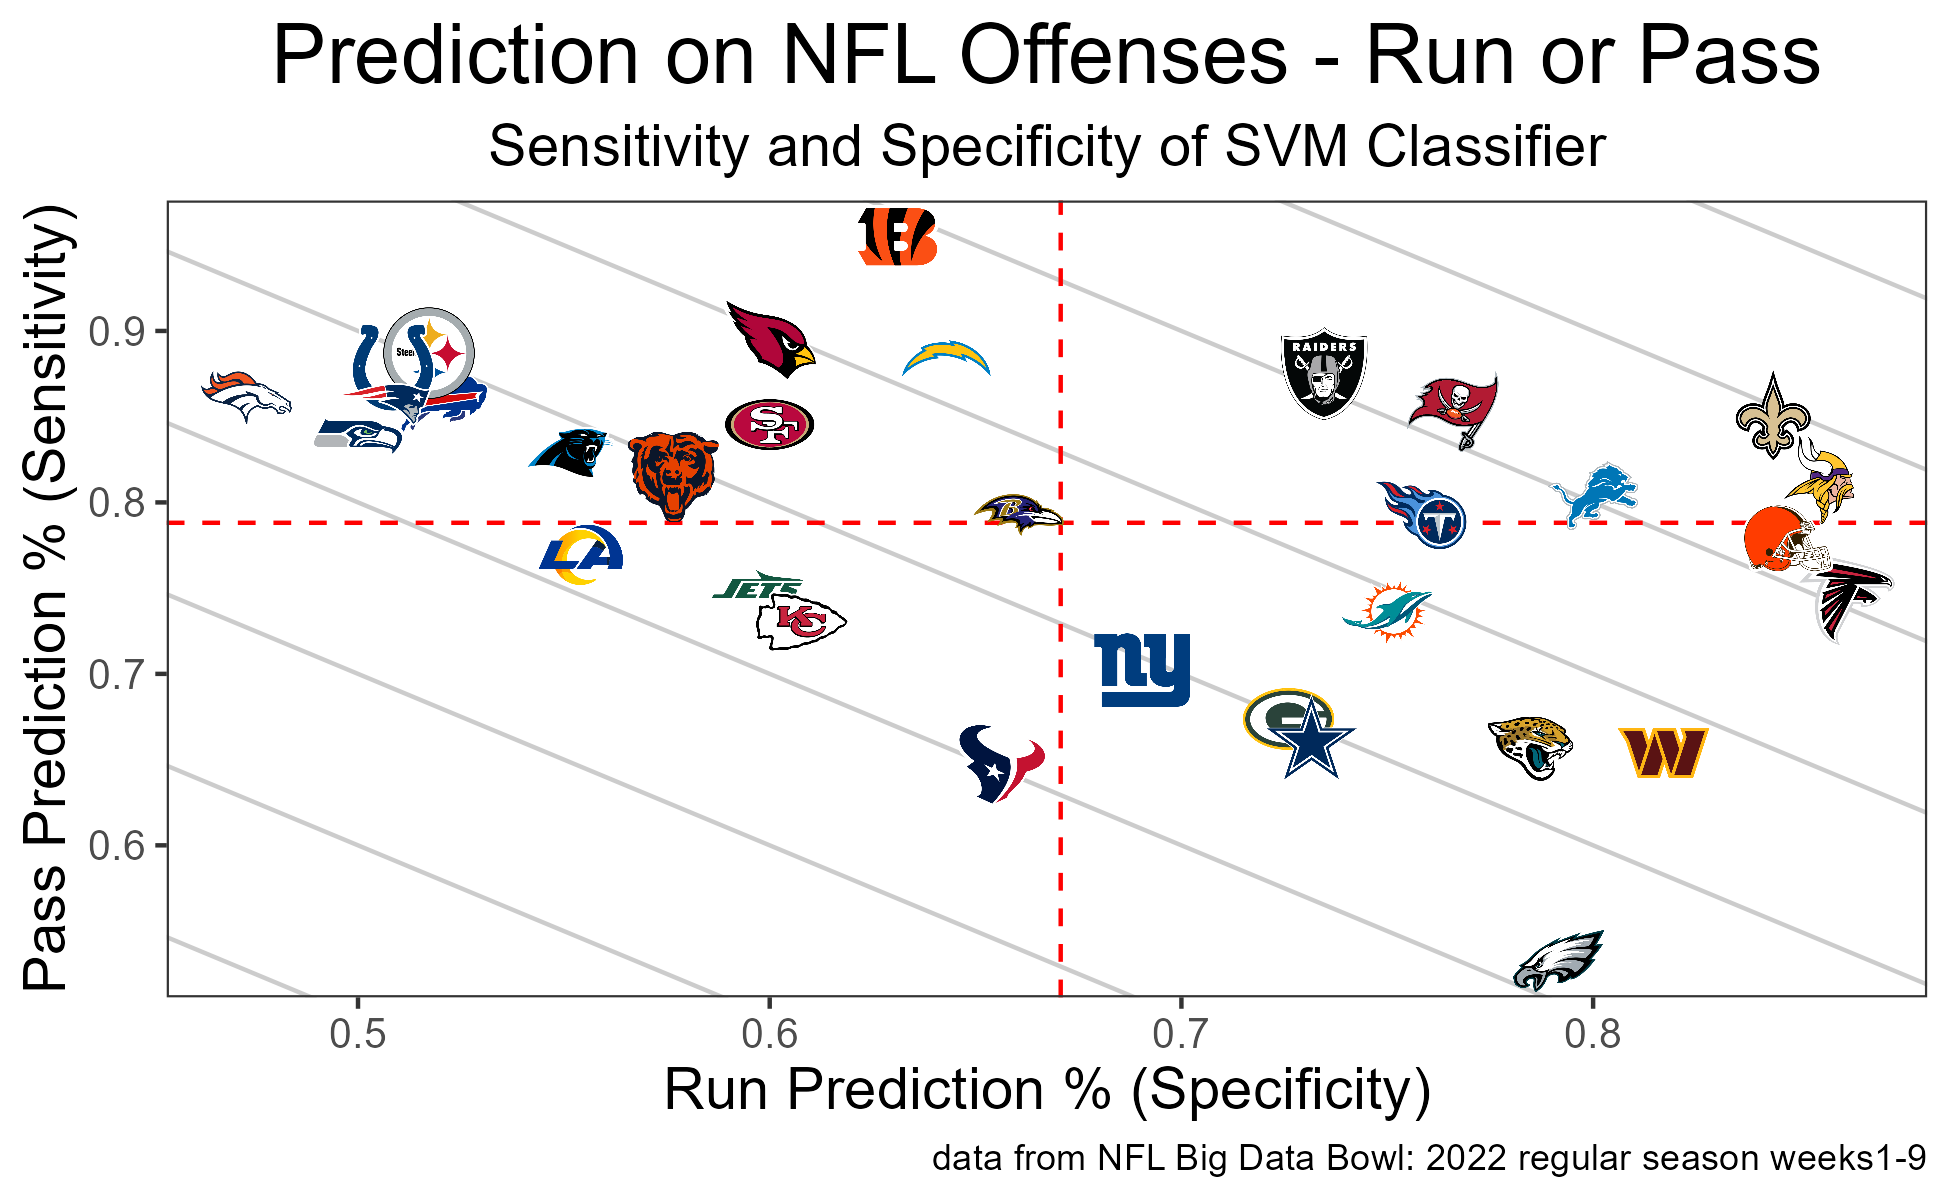
\includegraphics[width=27.08in]{graphs/Images for paper/SVM Specificity Sensitivity Graph - BW Theme}

When we look at the breakdown between run and pass predictions in the
Sensitivity vs Specificity plot, we can see a similar level of
predictability for each team. As mentioned each team has a different
proportion of run and pass plays, and this will influence the
predictability. However, there is a line to the bottom left of the plot
that no team falls below in. Almost a predictability minimum for the SVM
model indicating a high level of performance, even for the teams lower
in performance.

\subsection{9. Results- Random Forest:}\label{results--random-forest}

Preliminary model assessment included analyzing the best parameters for
each team to determine similarities and differences. I found that each
team varied widely in the optimal tuning parameters. For example, the
Los Angeles Chargers model had a mtry of 5 and a min.node.size of 1
while the Los Angeles Rams had mtry of 9 and min.node.size of 30. Though
the best tunes varied, I was surprised to see many teams with
min.node.size's of 1. This would indicate that deep trees were grown,
potentially overfitting. However, considering teams may have only been
trained on a couple hundred plays, this makes sense.

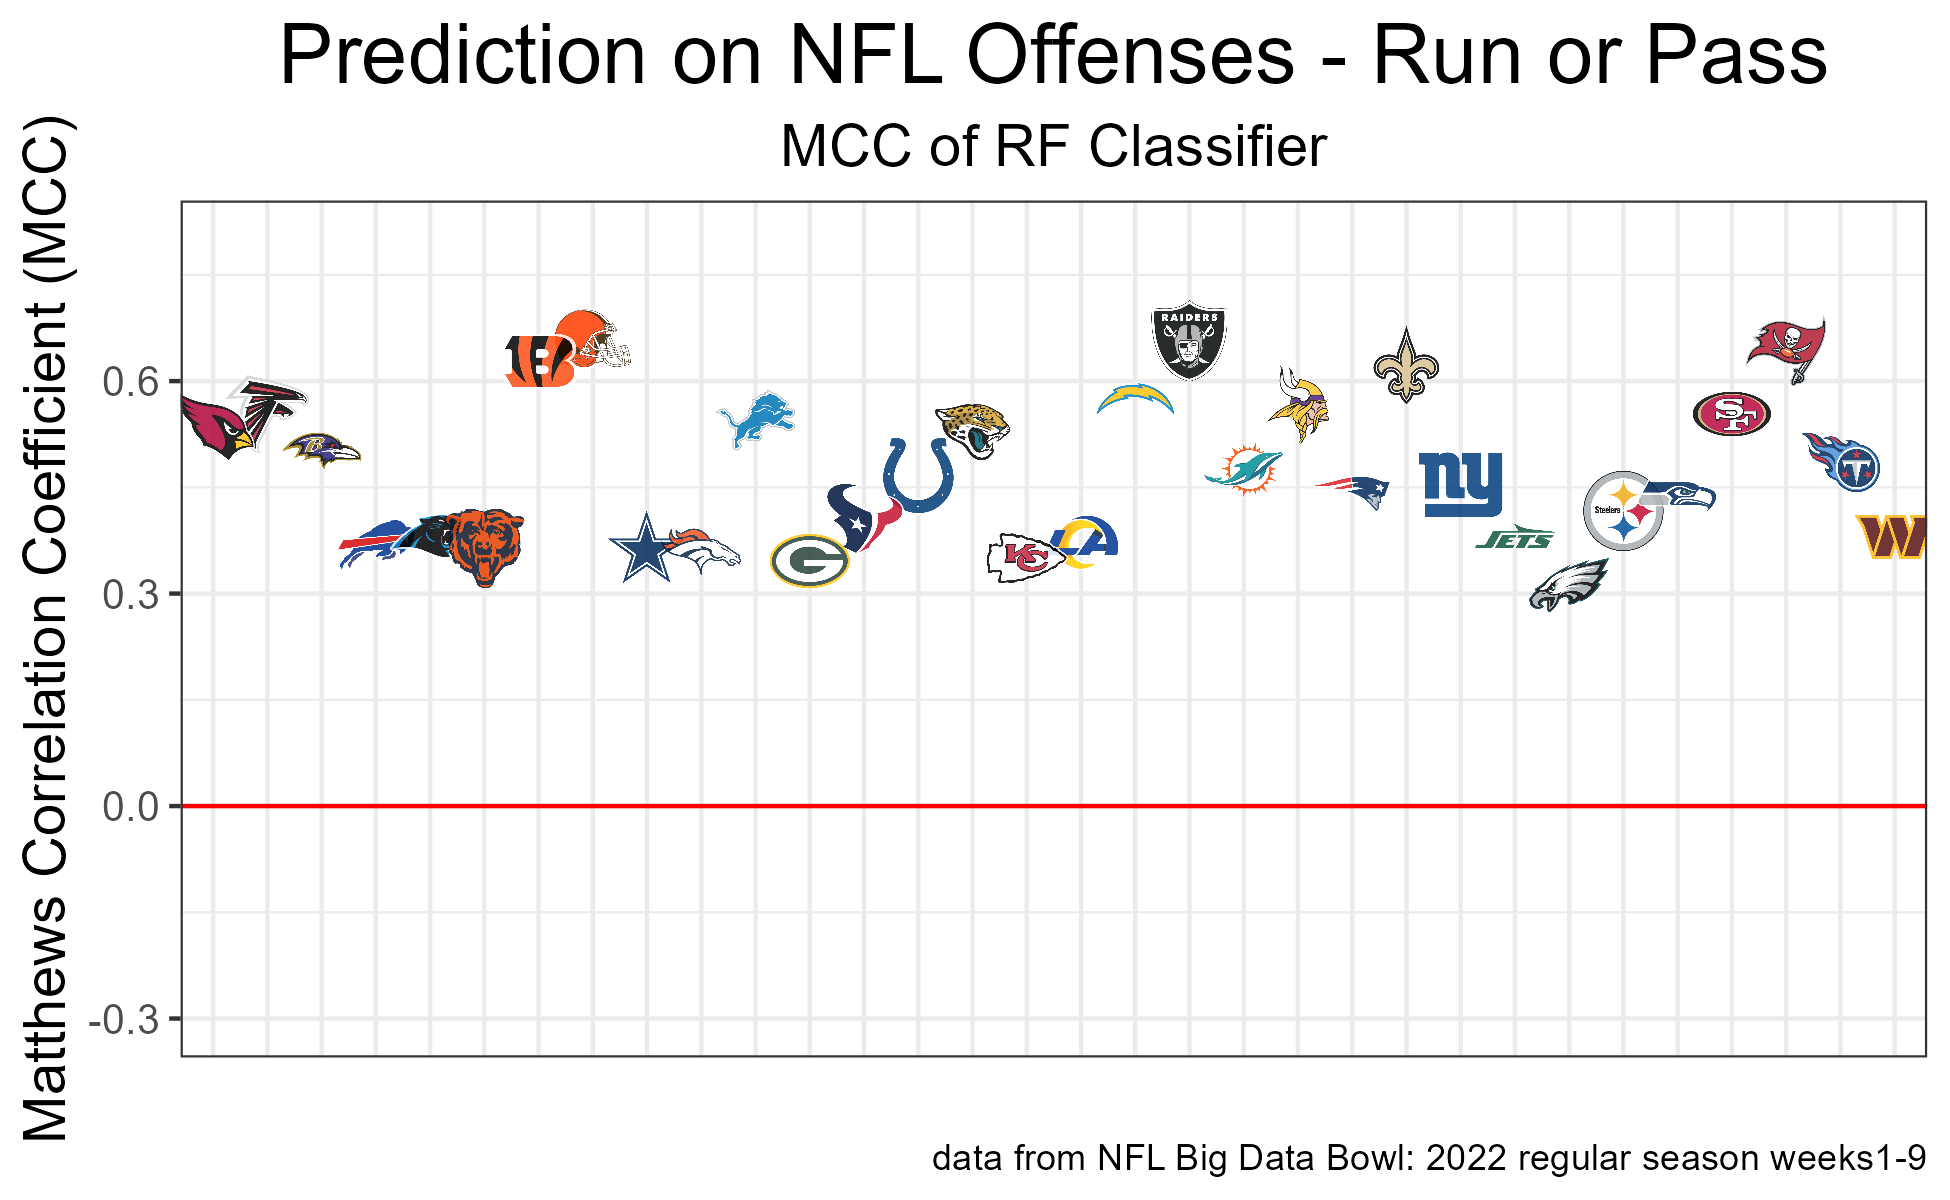
\includegraphics[width=27.08in]{graphs/Images for paper/final_mcc_rf}

As stated prior, to be able to compare model performance across models
we used Matthew's Correlation Coefficient(MCC). The performance of the
random forest model was very similar to the SVM model in terms of MCC.
All values for teams were above the value of 0.3, meaning that the
observed data and the predicted data positively agree.

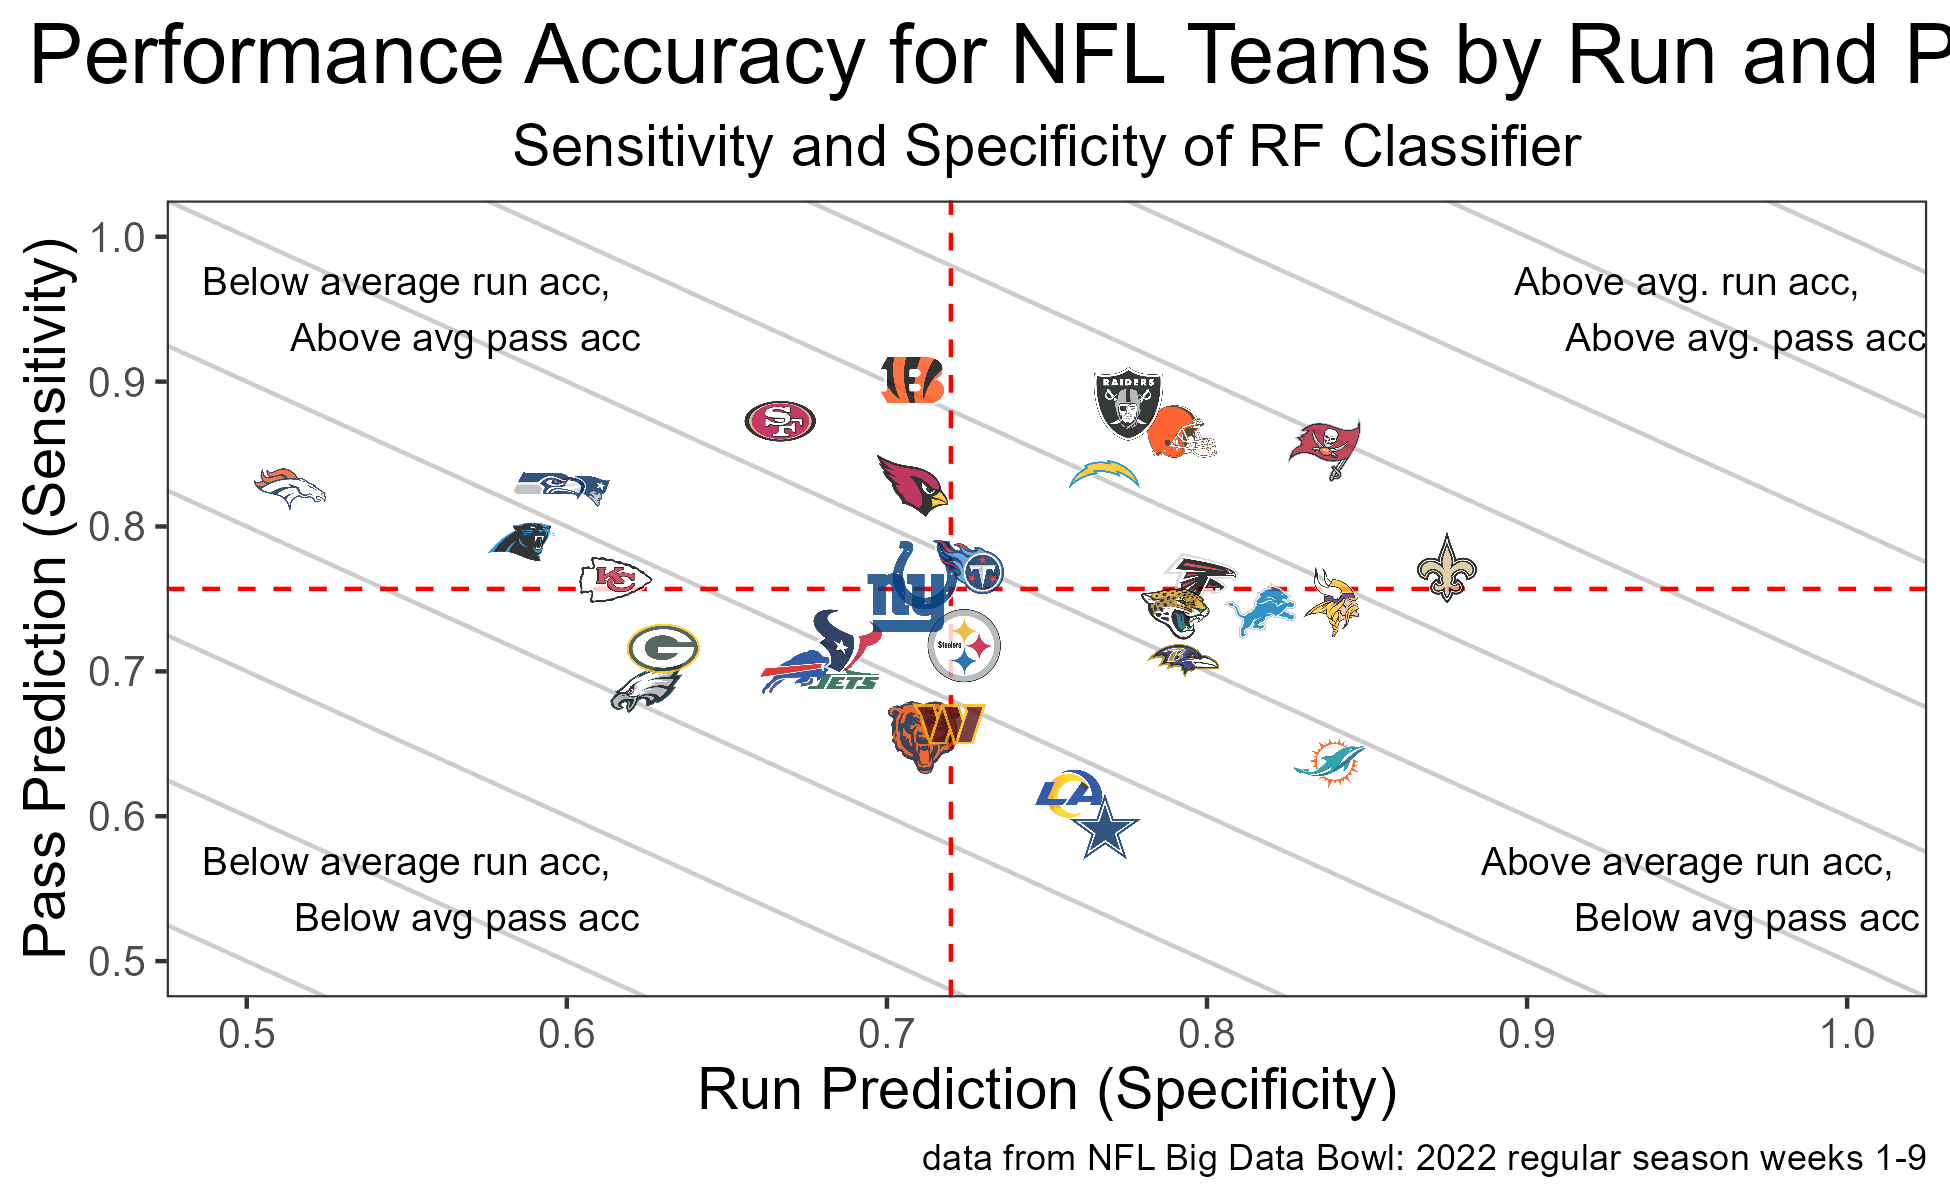
\includegraphics[width=27.08in]{graphs/Images for paper/final_sensspec_rf}

The random forest model provided promising results. When comparing
teams' test run play accuracy(specificity) and pass play
accuracy(sensitivity), we find that all values are above 0.5, proving we
can accurately predict much better than just a coin flip. We see in the
graph that there are not many outlier teams, with the teams forming a
circle around the means. This is encouraging to see that model
performance doesn't differ notably from team to team. Overall, the
predictions were quite accurate.

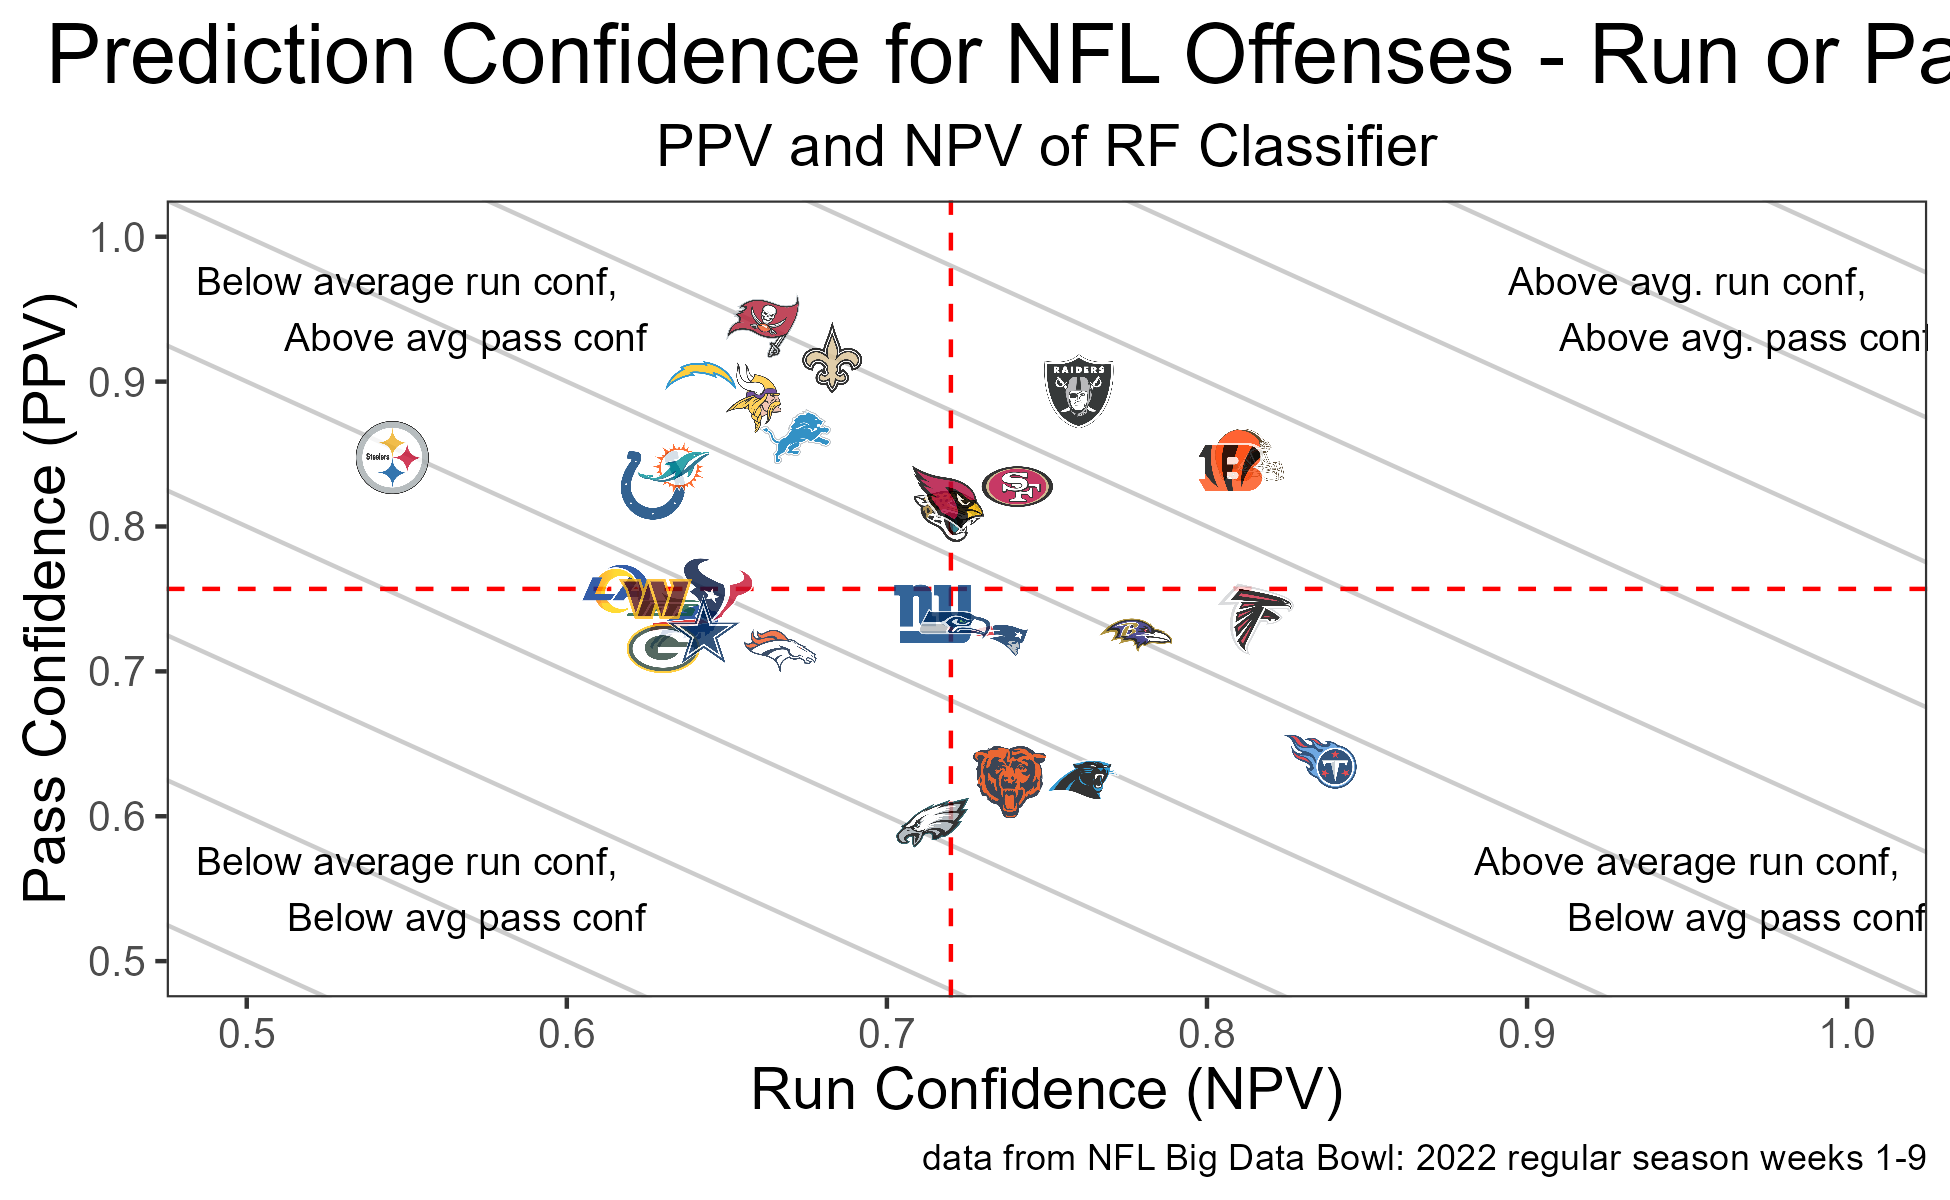
\includegraphics[width=27.08in]{graphs/Images for paper/final_predval_rf}

We can also see how confident we are in our predictions by evaluating
the passing predictive value(positive) and running predictive
value(negative). These values will tell us when we predict a certain
class, how certain we are in that predicted class.

Looking at the graph there are some interesting trends to pull from. We
notice that the team with the highest pass predictive value of 0.94, the
Tampa Bay Buccaneers, also had one of the highest pass play rates in the
league. With this, they have a below average run play predictive value
of 0.66, which is still a reasonable level of confidence. We can also
see that the four teams that ran more than passed(Tennessee Titans,
Atlanta Falcons, Philadelphia Eagles, Chicago Bears) are all located in
the bottom right quadrant. This quadrant represents above average run
play confidence and below average pass play confidence.

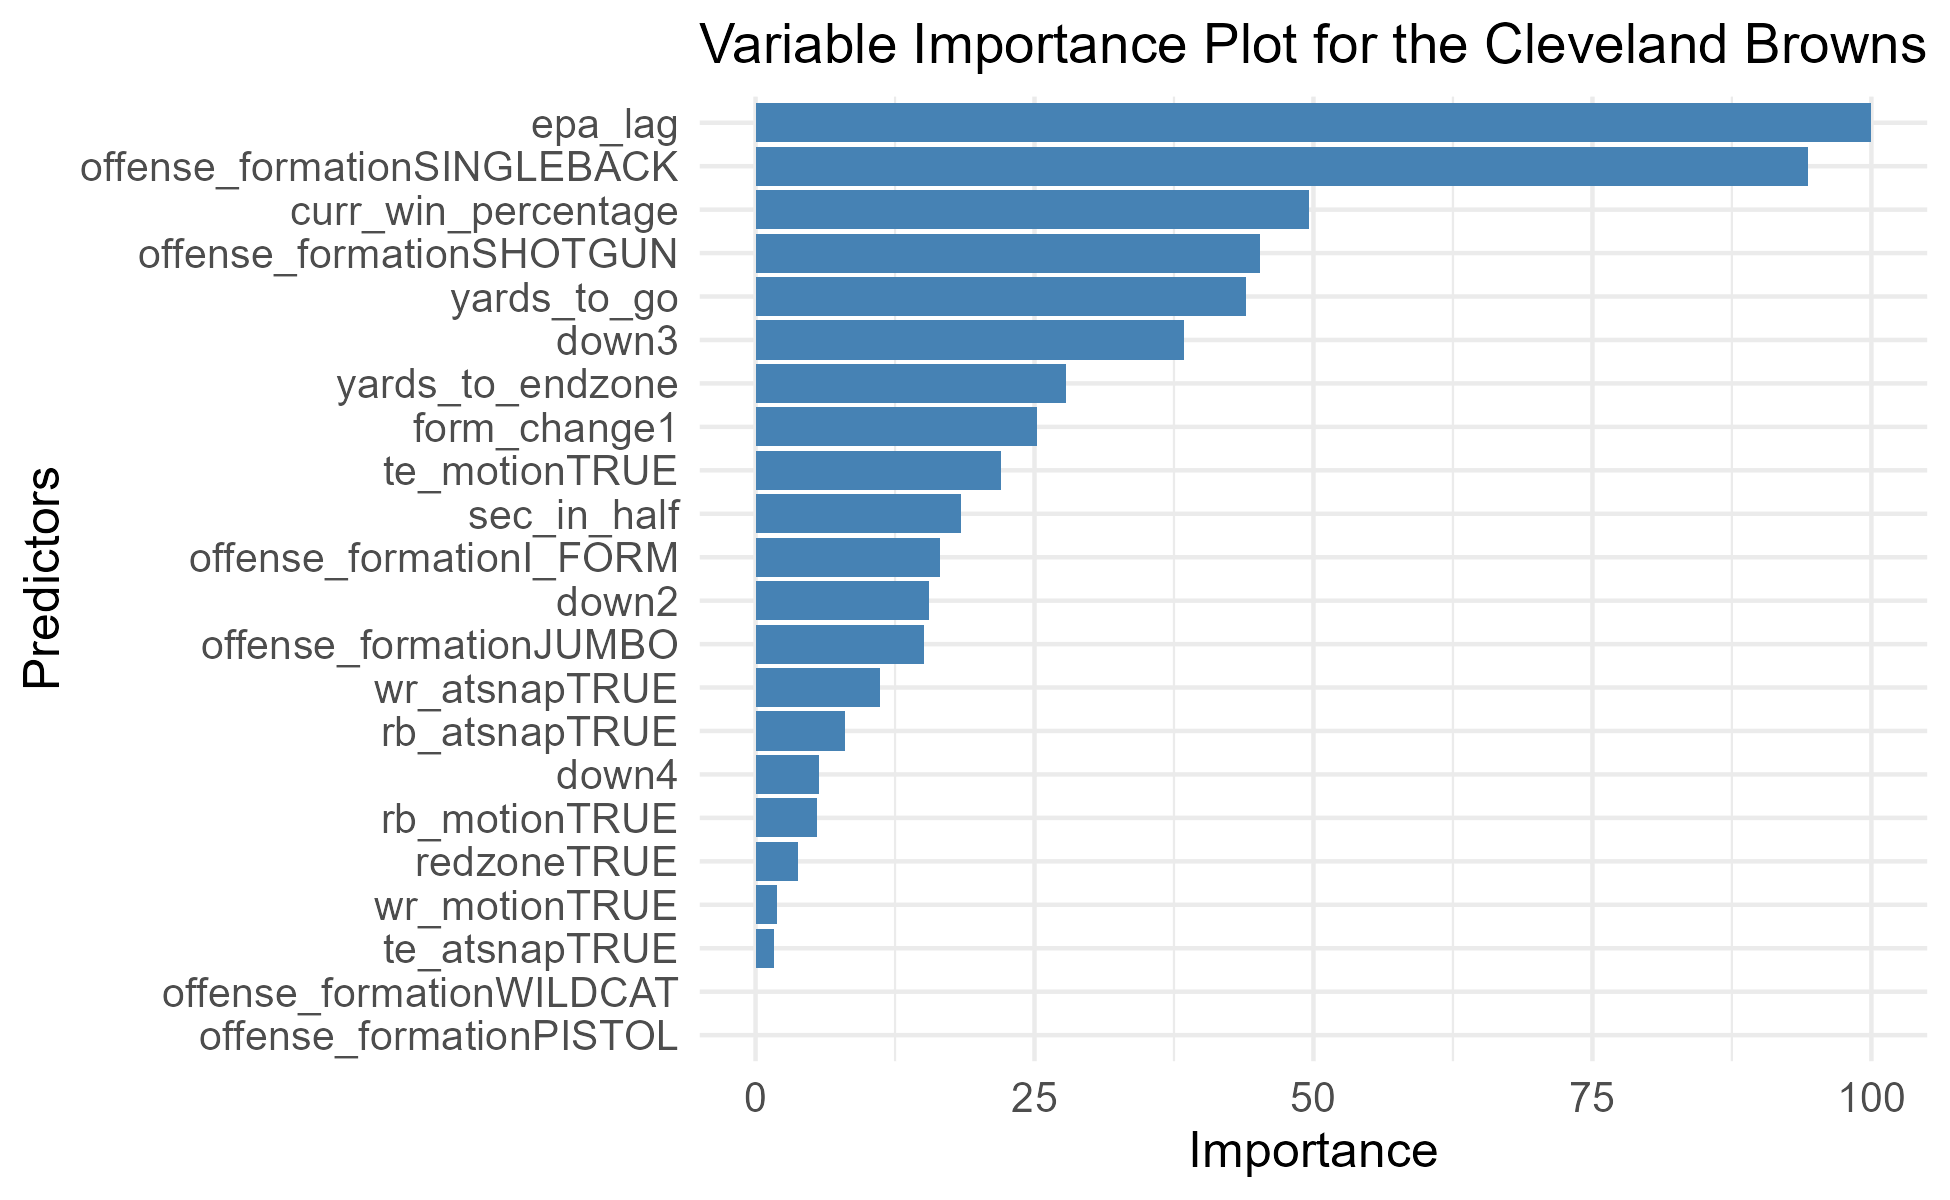
\includegraphics[width=27.08in]{graphs/Images for paper/final_CLEvar}
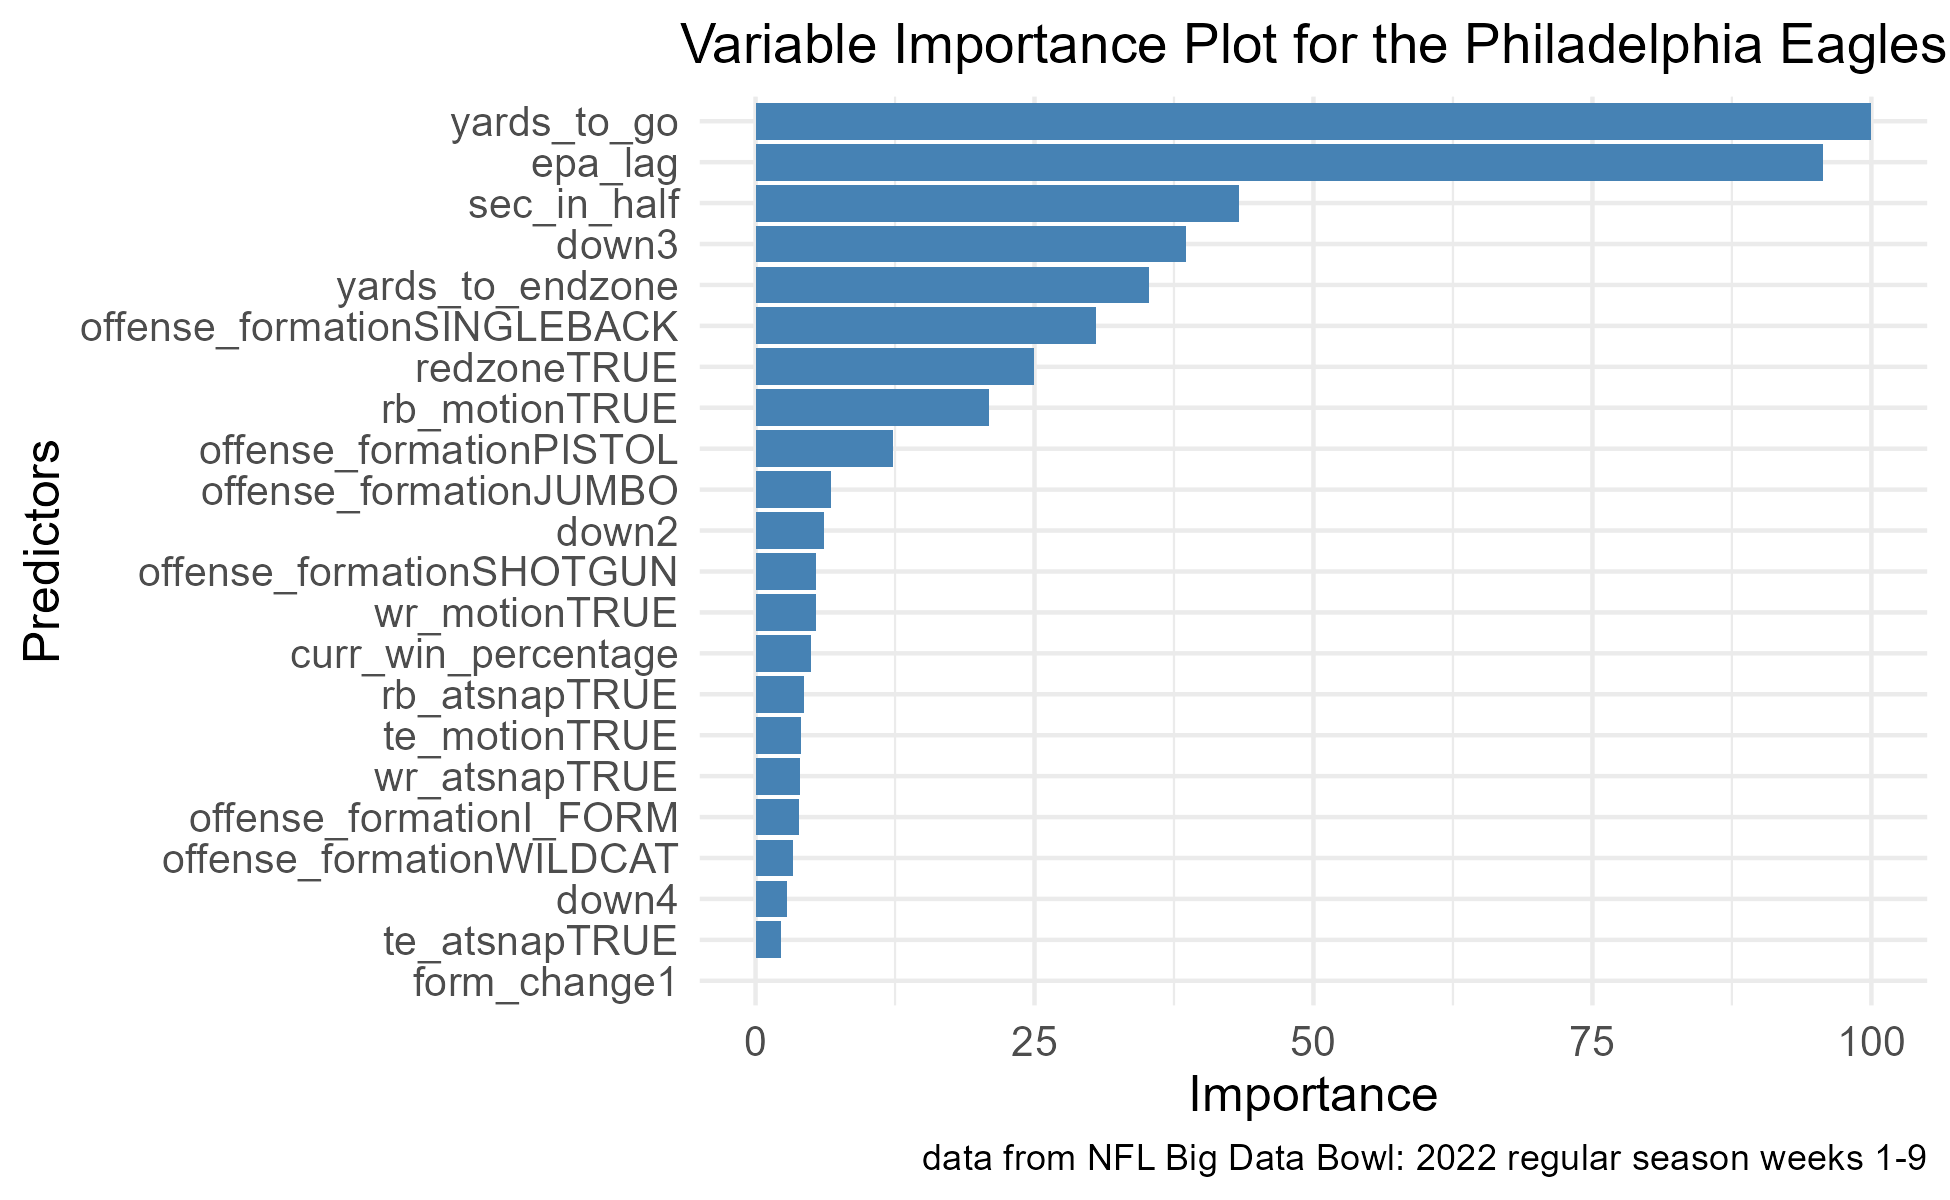
\includegraphics[width=27.08in]{graphs/Images for paper/final_PHIvar}

Given there are individual models for each team, the variable importance
across models may be drastically different. All teams have different
game plans which involve different formations, motions, prioritize
running or passing, and may react differently to different game
settings. To appreciate this we looked at the best and worst teams in
regard to their MCC values. These two teams are the Cleveland Browns
with an MCC of 0.66 and the Philadelphia Eagles with an MCC of 0.31. It
is interesting to see that both teams had epa lag(the measure of success
of the previous play) as one of the most important predictors. For the
Browns, it appears the model found formations that may signal whether
they pass or run. For the Eagles, it appears the model found trends in
different game settings(time left, yards to go, etc.) when determining
to pass or run.

\subsection{10. Model Comparison:}\label{model-comparison}

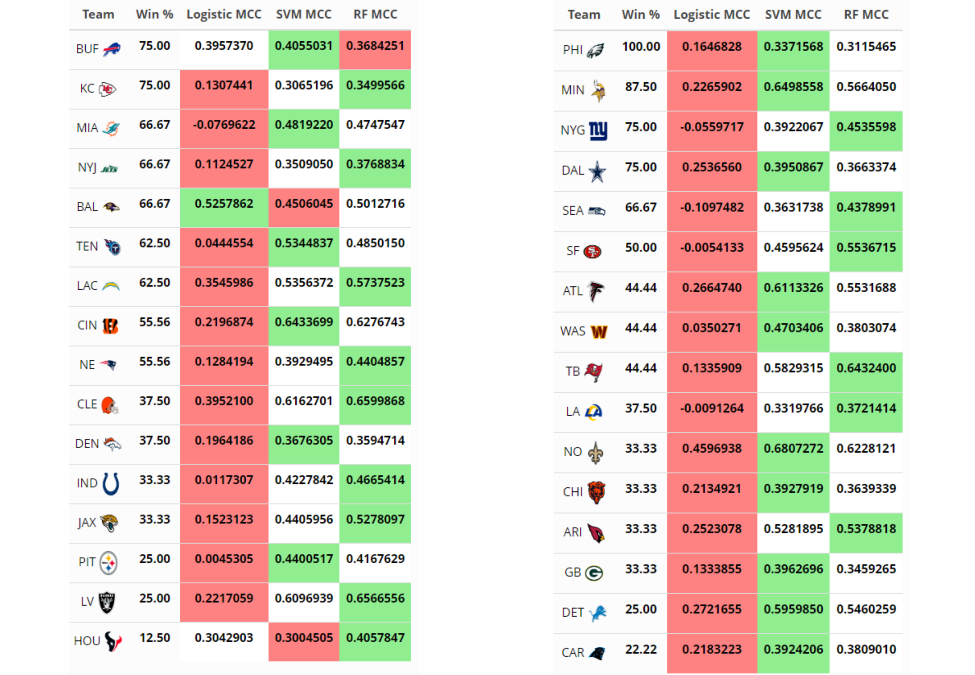
\includegraphics{Paper-RD_files/figure-latex/unnamed-chunk-14-1.pdf}

The above tables show the MCC values associated with each of our models
by team. Here the models with the highest (best) MCC scores are colored
in green while the lowest (worst) are colored in red. We can see that
the logistic regression model performed poorly compared to the Random
Forest and SVM with consistently lower MCC scores. The logistic model
had the highest MCC score only once for the Baltimore Ravens team.

The performance of the random forest and SVM models were much more
comparable with each having similar numbers of optimal MCC values. The
SVM model was the optimal model for 16 of the 32 teams with most scores
between 0.3 and 0.6. The random forest model was the optimal model for
15 of the 32 teams with most scores between 0.3 and 0.7. These findings
suggest that the random forest and SVM models are equally likely to be
the best choice, while the logistic regression model does not measure
up.

If we were to compare just the random forest to the SVM we can look at
the distribution of MCC values. The random forest had an average value
of 0.473 and a standard deviation of 0.105. The SVM had an average value
of 0.465 and a standard deviation of 0.112. Given these results, it
appears the random forest is performing better and is more stable across
teams.

\subsection{11. Conclusion:}\label{conclusion}

\subsection{12. Discussion and Future
Research}\label{discussion-and-future-research}

Currently, the predictions obtained from our models are solid. However,
we believe there are things that could be improved upon and explored.
Though many of the pre-play variables from the offenses perspective have
been covered, we neglected to consider the quality of our opponent. That
being said, there may be some opponent defensive performance metrics
that may be included in the model. For example, if we included the
ability of the opponents run and pass defense, that may give signal to
if the offense is better off running versus passing.

Other than including more predictors, we may also try different modeling
techniques. Specifically, we have considered evaluating different
kernels in our SVM models. Currently, we only evaluated the linear
kernel which has shown to be successful. However, the response we are
trying to predict may perform better with a more flexible decision
boundary such as the radial or polynomial kernel.

Separate from out offensive model, we would like to apply similar
methodologies to the defensive side of the ball. We could very easily
apply the same predictors we have(and more specific to the defensive
perspective) to predict whether a team will play zone coverage, man
coverage, blitz and more. This problem would introduce more response
classes and create a potentially more difficult problem.

\subsection{13. Citations:}\label{citations}

Michael Lopez, Thompson Bliss, Ally Blake, Paul Mooney, and Addison
Howard. NFL Big Data Bowl 2025.
\url{https://kaggle.com/competitions/nfl-big-data-bowl-2025}, 2024.
Kaggle.

H. Wickham. ggplot2: Elegant Graphics for Data Analysis. Springer-Verlag
New York, 2016. Carl S (2024). nflplotR: NFL Logo Plots in `ggplot2' and
`gt'. R package version 1.4.0.9001,
\url{https://github.com/nflverse/nflplotR},
\url{https://nflplotr.nflverse.com}.

DataScience-ProF. (2024, September 8). Understanding the Matthews
correlation coefficient (MCC) in machine learning. Medium.
\url{https://medium.com/@TheDataScience-ProF/understanding-the-matthews-correlation-coefficient-mcc-in-machine-learning-26e8049f8572\#}:\textasciitilde:text=The\%20MCC\%20can\%20be\%20understood,between\%20predictions\%20and\%20true\%20outcomes

\end{document}
